% !TeX root = ../main.tex
\chapter{Numerical investigation: preliminaries}
\label{chapt:results_preliminary}

\section{Inversion of the Dirac operator}
\label{sec:inversion_dirac}
As mentioned in section \ref{sec:langevin_monte_carlo}, the inversion of the Dirac operator is a computationally expensive operation. In fact, simple algorithms to invert a matrix such as Gaussian elimination have a computational complexity of $O(n^3)$ \cite{cond_num_ref}, while the best algorithm available nowadays has been proved to scale as $O(n^{2.371552})$ \cite{williams2023new}. \\
To circumvent this, since we are often only interested in applying the inverse matrix to a vector, we make use of the Conjugate Gradient algorithm, as detailed in appendix \ref{chap:AppendixC}. \\
We now want to give an idea of the speed-up that one can gain by following such approach, keeping in mind that this is an operation which has to be performed at each evolution step.  \\
To do this, we construct a Dirac operator described by equation \eqref{eq:wilson-dirac_operator} with bare quark mass $m_q = 0.5$ and Yukawa coupling $g=0.5$. We then add a fluctuating scalar field 
\begin{equation*} 
    \phi(x) = v + \eta(x),
\end{equation*} 
where $v = 1.0$ and $\eta$ is a normally distributed number with mean $0$ and unitary variance. \\
We then measure the time needed to compute 
\begin{equation*}
    \xi = D^{-1}\psi,
\end{equation*}
where $\psi$ is a vector of random numbers uniformly ditributed between $-1$ and $1$. We study the time dependence as a function of the vector size $V$ by averaging over 20 measures per each value of $V$. \\
Figure \ref{fig:complexity} reports the results of the experiment. Assuming that our algorithm has complexity $O(V^b)$, namely that when $V \to \infty$,
\begin{equation*}
    t \approx a \, V^b,
\end{equation*}
we fit our data according to the model 
\begin{equation*}
    \log t = \log a + b \log V.
\end{equation*}
We find 
\begin{equation*}
    \log a = -3.1 \pm 0.1 \qquad b = 1.02 \, \pm 0.02.
\end{equation*}
Note that for a standard Gaussian elimination procedure we would have found $b \approx 3.0$. This is of particular relevance in the case of this work, since the cooling technique via coloured noise requires doubling the number of lattice points in each direction at each block spin step; hence the volume of the lattice is increased by a factor $2^d$ at each iteration, where $d$ is the spacetime dimension. \\
Typical lattices sizes in this work are up to $128 \times 128 \times N_f \times N_s \approx 10^5$, where $N_f$ is the number of flavours and $N_s$ is the number of spinor components. Therefore, a good volume scaling of the algorithm is strictly necessary.
\begin{figure}[t]
    \centering
    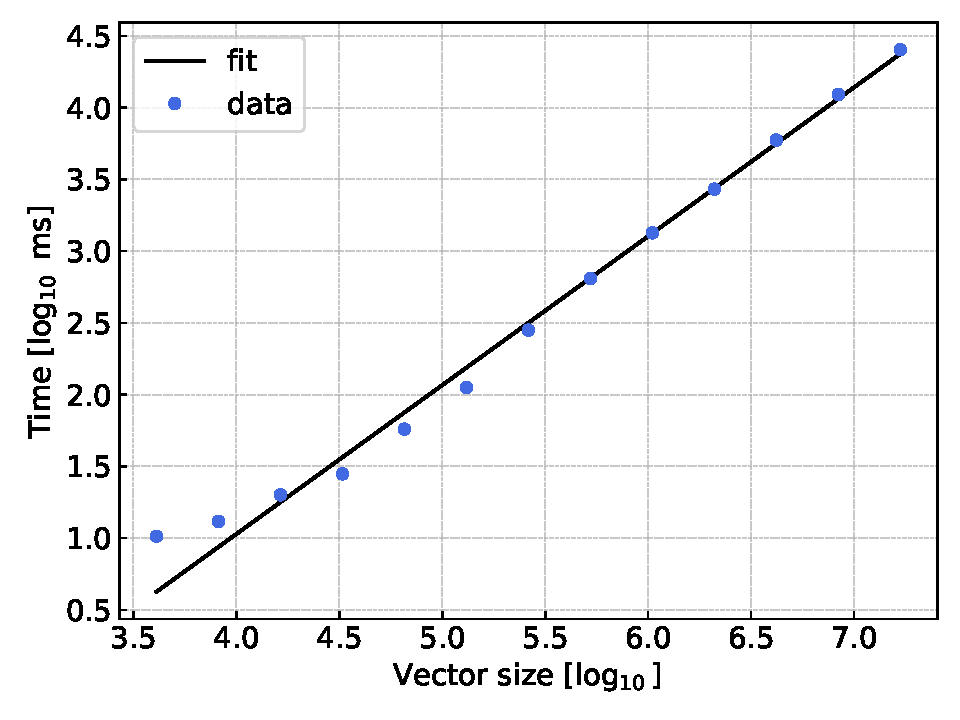
\includegraphics[scale=0.65]{figures/complexity.pdf}
    \caption[Computational complexity of the Conjugate Gradient algorithm.]{Computational complexity of the Conjugate Gradient algorithm in our model. The results show the operation time scales as $t \sim \mathcal{O}(V^{1.03})$ for large verctor sizes, while for a standard inversion via Gaussian elimination one would have $t \sim \mathcal{O}(V^3)$.}
    \label{fig:complexity}
\end{figure}

\section{The fermionic correlator}
We now want to analyse the behaviour of the fermionic correlator and illustrate the fermionic masses extraction procedure. \\
Let us for the moment restrict to $g = 0$, so that the Dirac operator reduces to the one of free Wilson fermions 
\begin{equation}
    \begin{aligned}
    \widehat{D}_{m, n} = &- \left(\frac{\Gamma_{+\hat 0}}{2} \, \delta_{m, m+\hat 0} +\frac{\Gamma_{-\hat 0}}{2} \, \delta_{m, m-\hat 0} + \frac{\Gamma_{+\hat 1}}{2} \, \delta_{m, m+\hat 1} + \frac{\Gamma_{- \hat 1}}{2} \, \delta_{m, m-\hat 1}\right)  \\
     &+ \left(2ar + \hat m \right) \, \delta_{s,s'} \, \delta_{m,n}. \\
    \end{aligned}
    \label{eq:wilson-dirac_operator_free}
\end{equation}
We then compute the correlator \eqref{eq:correlator_func} numerically via a single inversion of the Dirac operator using the Conjugate Gradient algorithm as detailed in Appendix \ref{chap:AppendixC}. The lattice volume is chosen to be $128 \times 128$. \\~\\
Figure \ref{fig:correlator_mass} reports the fermionic correlator as a function of $m_q$. One can see that a bigger bare quark mass results in a quicker decay, according to the decay law 
\begin{equation*}
    \lim_{t \to \infty} \expect{\psi(t)\bar\psi(t)}_{s,s'} \propto e^{-m_\text{phys} \, t}.
\end{equation*}
On the other side, a smaller mass results in a slower decay and tends to deform the characteristic shape of the correlator.
\begin{figure}[h]
    \centering 
    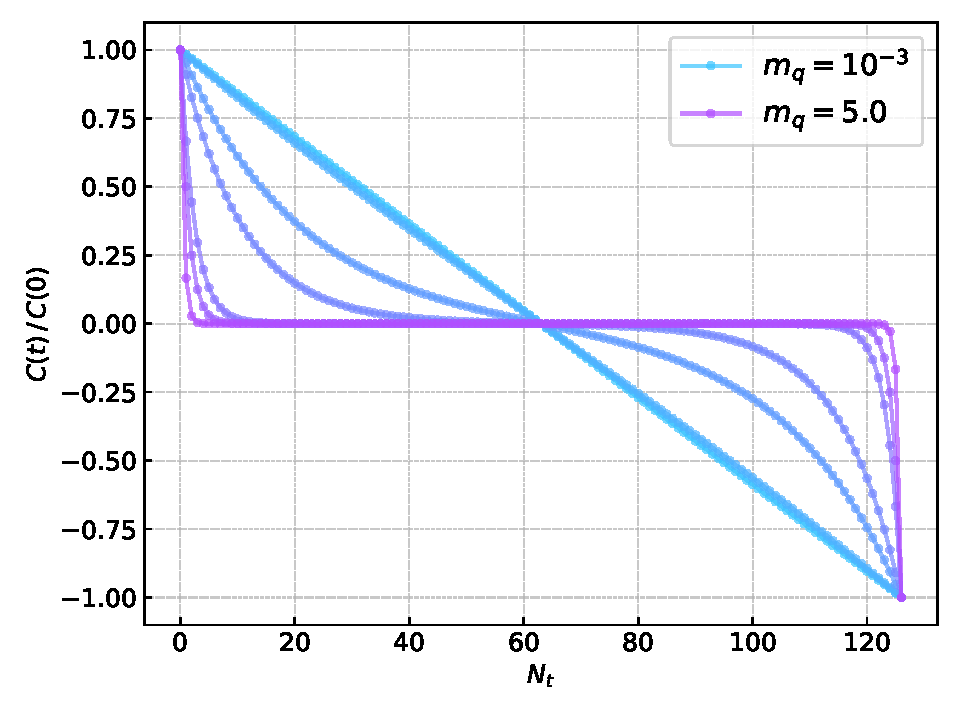
\includegraphics[scale=0.6]{figures/correlator/correlator.pdf}
    \caption[Fermionic correlator]{Normalised fermionic correlator for different values of the bare quark mass. A bigger mass results in a quicker decay of the correlator.}
    \label{fig:correlator_mass}
\end{figure}\\
Figure \ref{fig:correlator_CGiter} shows the number of iterations needed for convergence of the Conjugate Gradient algorithm. While the exact number depends on the desired tolerance, one can clearly see that the number of iterations grows as $m_q \to 0$, due to an increase in the condition number \cite{cond_num_ref}. \\
\begin{figure}[h!]
    \centering 
    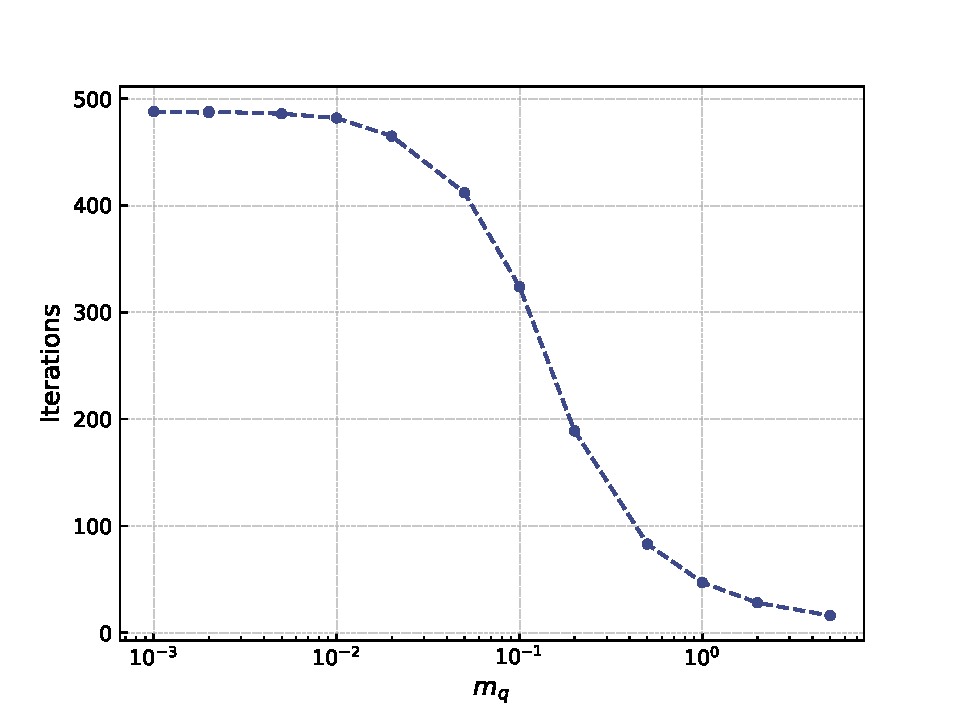
\includegraphics[scale=0.6]{figures/correlator/CGiter.pdf}
    \caption[Conjugate Gradient algorithm iterations as a function of the bare quark mass.]{Conjugate Gradient algorithm iterations as a function of the bare quark mass. As $m_q \to 0$ the number of iterations grows due to an increase in the condition number.}
    \label{fig:correlator_CGiter}
\end{figure} \\
For the Dirac operator \ref{eq:wilson-dirac_operator_free}, one can derive an analytical expression for the physical mass, the pole of the propagator. \\
To do this, let us consider the momentum space expression of the Dirac operator, which is derived in appendix \ref{chap:AppendixB}
\begin{equation*}
\bar{D}(p)= \hat{m}_q + \sum_\mu 2 \sin ^2\left(\frac{p_\mu \, a}{2}\right)+i \sum_\mu \gamma_\mu \sin \left(p_\mu \, a\right).
\end{equation*}
This can be straightforwardly inverted to
\begin{equation*}
    \bar{D}^{-1}(p) = \frac{\hat{m}_q + \sum_\mu 2 \sin ^2\left(\frac{p_\mu \, a}{2}\right) - i \sum_\mu \gamma_\mu \sin \left(p_\mu \, a\right)}{\hat{m}_q + \sum_\mu 2 \sin^2\left(\frac{p_\mu \, a}{2}\right) + \sum_\mu \sin^2 \left(p_\mu \, a\right)}.
\end{equation*}
One can now find the pole by imposing the denominator evaluated at $p^\mu =(im_\text{phys}, 0)$ to zero:
\begin{equation*}
    \left[\hat{m}_q + \sum_\mu 2 \sin ^2\left(\frac{p_\mu \, a}{2}\right)\right]^2_{p_\mu = (im_\text{phys}, 0)} + \left[\sum_\mu \gamma_\mu \sin \left(p_\mu \, a\right)\right]^2_{p_\mu = (im_\text{phys}, 0)} = 0.
\end{equation*}
This results in a trascendental equation 
\begin{equation*}
    \left[\hat{m}_q - 2 \sinh^2\left(\frac{\hat{m}_\text{phys}}{2}\right)\right]^2 - \sinh^2\left(\hat{m}_\text{phys}\right) = 0,
\end{equation*}
which has the solution 
\begin{equation}
    \hat{m}_\text{phys} = \log\left(1+\hat{m}_q\right).
    \label{eq:analytical_wilson}
\end{equation}
We then choose three values of the bare quark mass, compute the correlator numerically and perform a fit according to \eqref{eq:correlator_func}, in order to extract the physical mass. We then compare it to the theoretical value given by \eqref{eq:analytical_wilson}. The results are reported in figures \ref{fig:fit_wilson} and table \ref{tab:free_wilson_fit}. \\~\\
Note that in an interacting theory, excited states are, strictly speaking, negligible only for $t \to \infty$. This means that they may affect the characteristic shape of the correlator, and one has to either consider only a smaller window centered around $t=N/2$, or to make a fit to a portion of the exponential decay, in order to extract the mass \textcolor{blue}{I might try to bring an example}.
\newpage
\begin{table}[h!]
    \centering
    \begin{tabular}[pos]{ccc}
        \toprule
        $m_q$ & teo & fit \\
        \midrule 
        1.0 & 0.6931471805599453 & 0.6931537171644739 \\
        0.1 & 0.09531017980432493 & 0.09531020915059212 \\
        0.01 & 0.009950330853168092 & 0.009950277657505842 \\
        \bottomrule
    \end{tabular}
    \caption[Fit of the correlator for free Wilson fermions.]{The correlator for free Wilson fermions is fitted to equation \eqref{eq:correlator_func} and compared to its analytical value given by \eqref{eq:analytical_wilson}. The precision for the Conjugate Gradient algorithm was set to $r^2 \leq 10^{-10}$.}
    \label{tab:free_wilson_fit}
\end{table}
\begin{figure}[h!]
    \centering
    \begin{subfigure}[b]{0.47\textwidth}
        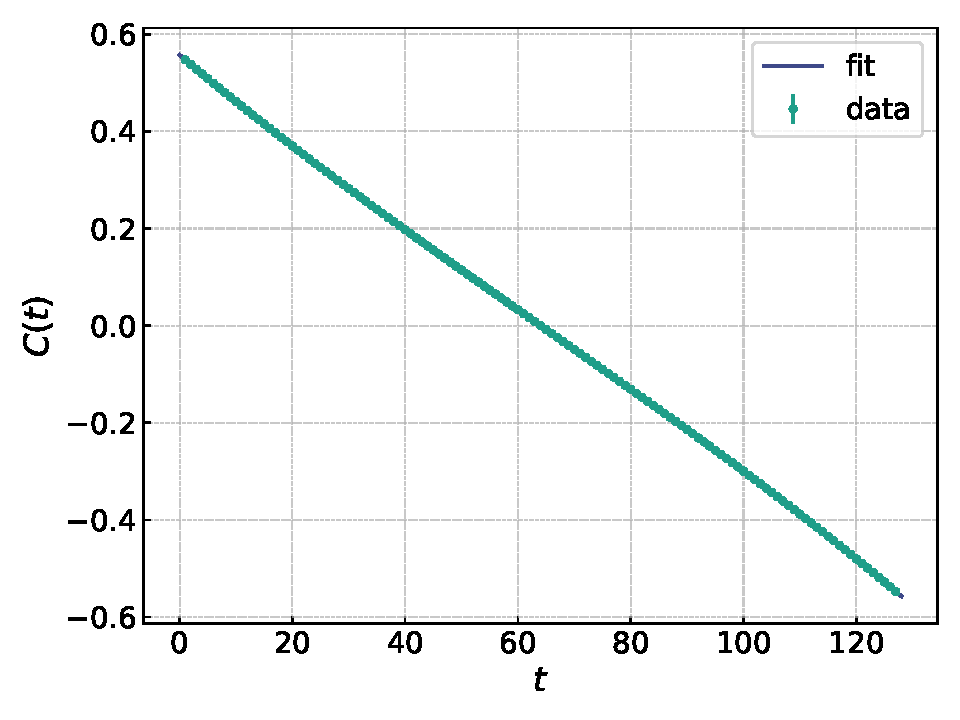
\includegraphics[width=\textwidth]{figures/correlator/corrs_free/corr_small.pdf}
        \caption{$m_q = 0.01$}
    \end{subfigure}
    \hfill
    \begin{subfigure}[b]{0.47\textwidth}
        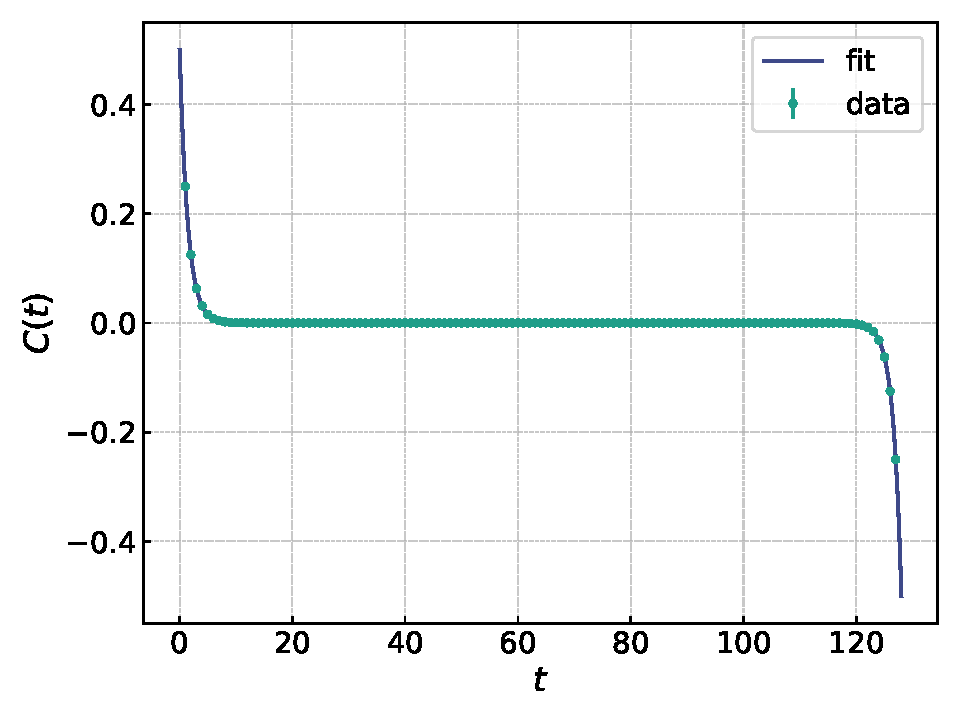
\includegraphics[width=\textwidth]{figures/correlator/corrs_free/corr_big.pdf}
        \caption{$m_q = 1.0$}
    \end{subfigure}
    \\
    \vspace{10pt}
    \begin{subfigure}[b]{0.68\textwidth}
        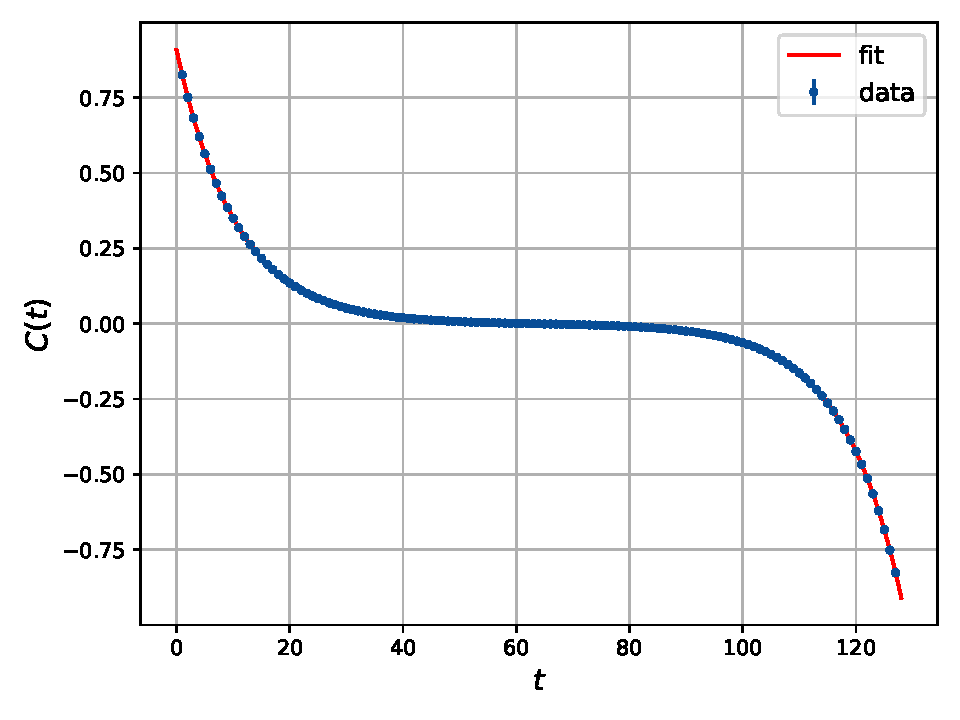
\includegraphics[width=\textwidth]{figures/correlator/corrs_free/corr_medium.pdf}
        \caption{$m_q = 0.1$}        
    \end{subfigure}
    \caption[Fit of the correlator for free Wilson fermions.]{Fit of the fermionic correlator acording to equation \eqref{eq:correlator_func}, for three different values of the bare quark mass. \\ The results are reported in table \ref{tab:free_wilson_fit}.}
    \label{fig:fit_wilson}
\end{figure}

\newpage

\section{Phase structure}
We want to start the analysis of the Yukawa theory by doing a parameters scan, in order to have a global picture of the phase diagram in the presence of Wilson fermions. For the remaining of this section, we set the value of the fermionic bare mass to $m_q = 1.0$.\\~\\
Figure \ref{fig:phase_diagram_g_m} reports a slice of the phase diagram in the $g-m_\phi^2$ plane. \\
For $g=0$, the fermionic and bosonic theories are independent. In particular the scalar theory reduces to a O(1) interacting theory: for $m_\phi^2>0$ the system lies in a symmetric state identified by $\expect{\phi} = 0$. 
As the mass goes to negative values, the scalar field gains a non-zero expectation value, signaling the spontaneous breaking of the O(1) symmetry. \\
When a finite Yukawa coupling is added, the finite bare quark mass and the Wilson term, that break chiral symmetry explicitly, are fed to the scalar field, which gains a vacuum expectation value due to the relation \eqref{eq:qualitative_relation_condensate_magnetisation_mass}.
\begin{figure}[htp]
    \centering
    \begin{subfigure}[b]{0.47\textwidth}
        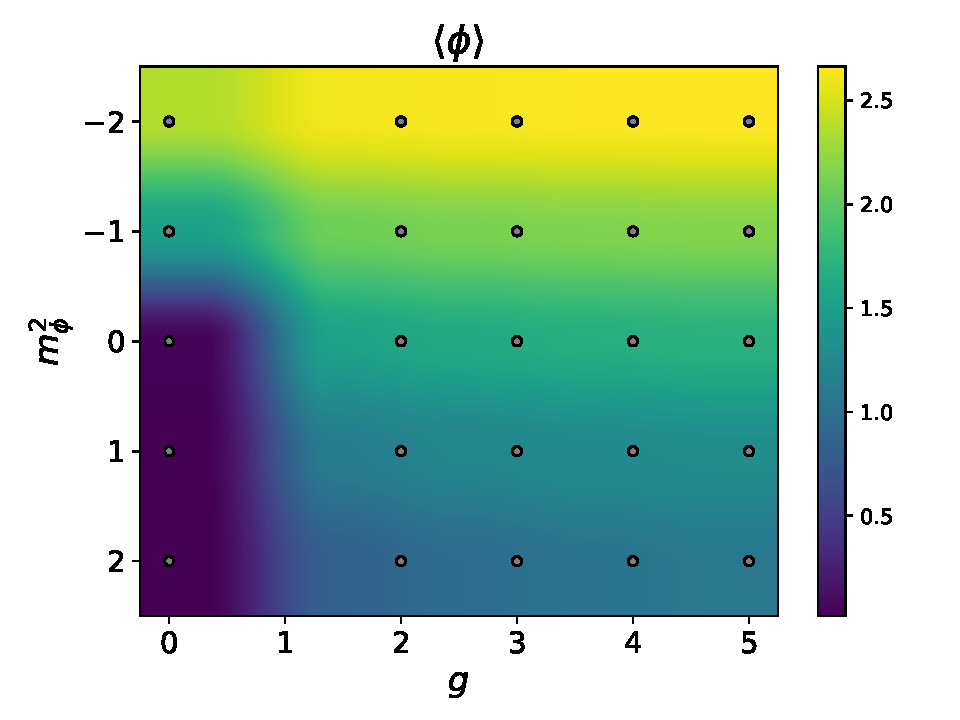
\includegraphics[width=\textwidth]{figures/phase_diagram/g-m/phase_diagram_phi.pdf}
    \end{subfigure}
    \begin{subfigure}[b]{0.47\textwidth}
        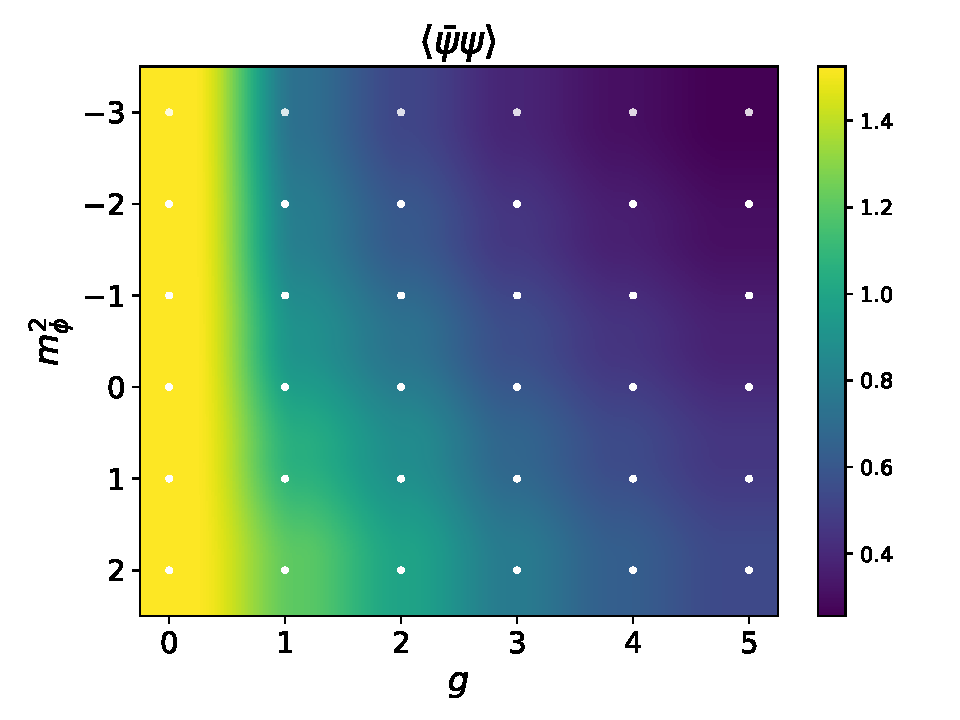
\includegraphics[width=\textwidth]{figures/phase_diagram/g-m/phase_diagram_cond.pdf}
    \end{subfigure}
    \begin{subfigure}[b]{0.47\textwidth}
        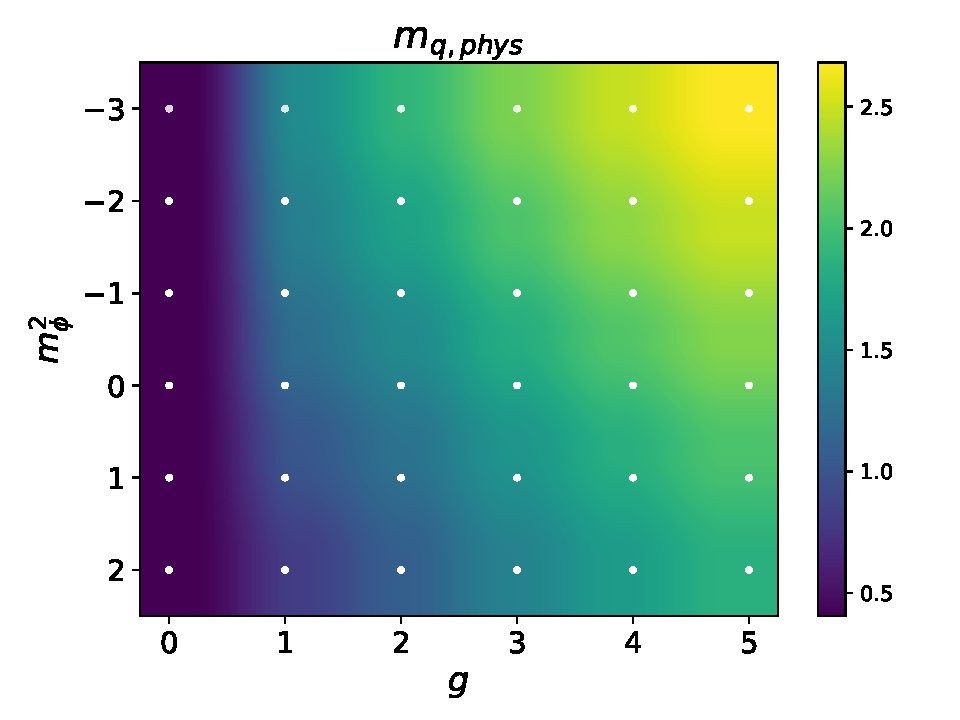
\includegraphics[width=\textwidth]{figures/phase_diagram/g-m/phase_diagram_mqphys.pdf}
    \end{subfigure}
    \begin{subfigure}[b]{0.47\textwidth}
        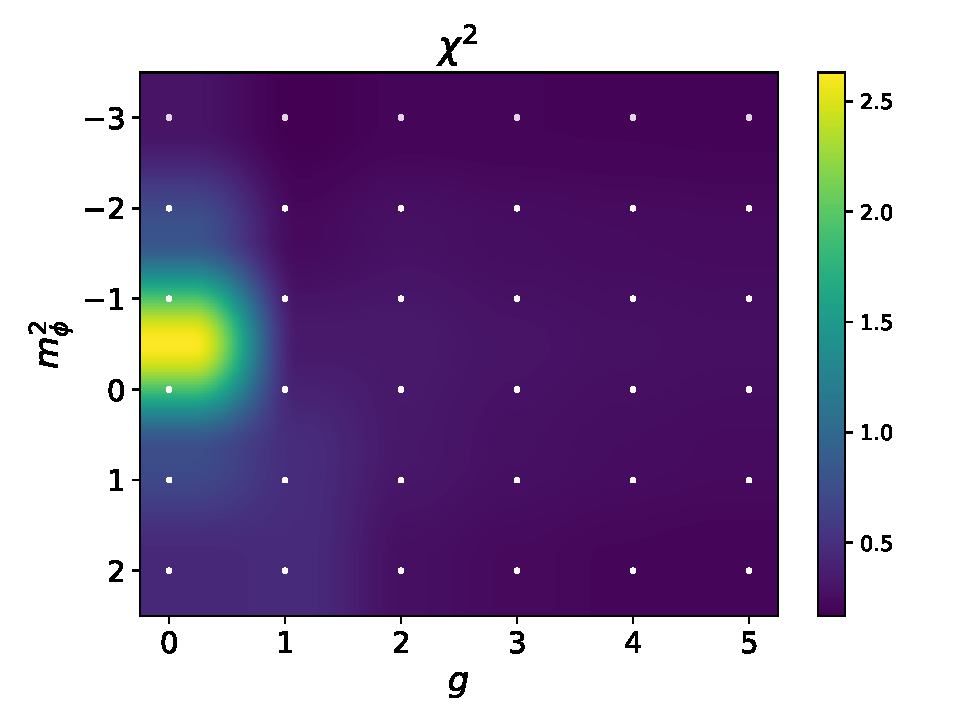
\includegraphics[width=\textwidth]{figures/phase_diagram/g-m/phase_diagram_chi2.pdf}
    \end{subfigure}
    \caption{Slice of the phase diagram at fixed $\lambda = 2.0$. \\ Lattice size $32 \times 32$, $N_\text{conf} \approx \mathcal{O}(5 \cdot 10^4)$.}
    \label{fig:phase_diagram_g_m}
\end{figure}\\
The plot of the chiral condensate shows that chiral symmetry is always broken in the model, even for $g=0$. Because of this, for $g \neq 0$, one can never speak of a proper phase transition. Thus, one still have a smooth crossover between the two phases. This fact is reflected in the plot of the magnetic susceptibility, which peaks around $m_\phi^2 = 0$ only for small values of $g$. \\
As explained in section \ref{sec:Yukawa_theory}, the presence of a background scalar field can be interpreted as a bare quark mass. This is reflected in the plot of of $m_{q, \text{phys}}$ which resembles the one of $\expect{\phi}$, except for $g=0$, since the two theories are disconnected. \\~\\
Figure \ref{fig:phase_diagram_g_lam} reports the phase diagram in the $\lambda - g$ plane. The behavior can be understood qualitatively by means of classical arguments. 
For $g=0$, one expects a field magnetisation of order 
\begin{equation*}
    v = \sqrt{-\frac{6 m_\phi^2}{\lambda}}.
\end{equation*}
Hence, as $\lambda$ is increased, the expectation value of the field is reduced.
If $g \neq 0$, the fermion mass and the Wilson term contributions increase the expectation value of the field, which in turn works as an additional bare quark mass, hence increasing $m_{q, \text{phys}}$. The behavior of the susceptibility is analogous to the previous case: only if $g=0$ one has a proper phase transition, reflected in the single peak.
The precise value of $\lambda$ at which this happens depends, mainly, on the choice of $m_\phi^2$. \textcolor{red}{maybe do a scan also for $m_\phi^2 > 0$}
\begin{figure}[htp]
    \centering
    \begin{subfigure}[b]{0.47\textwidth}
        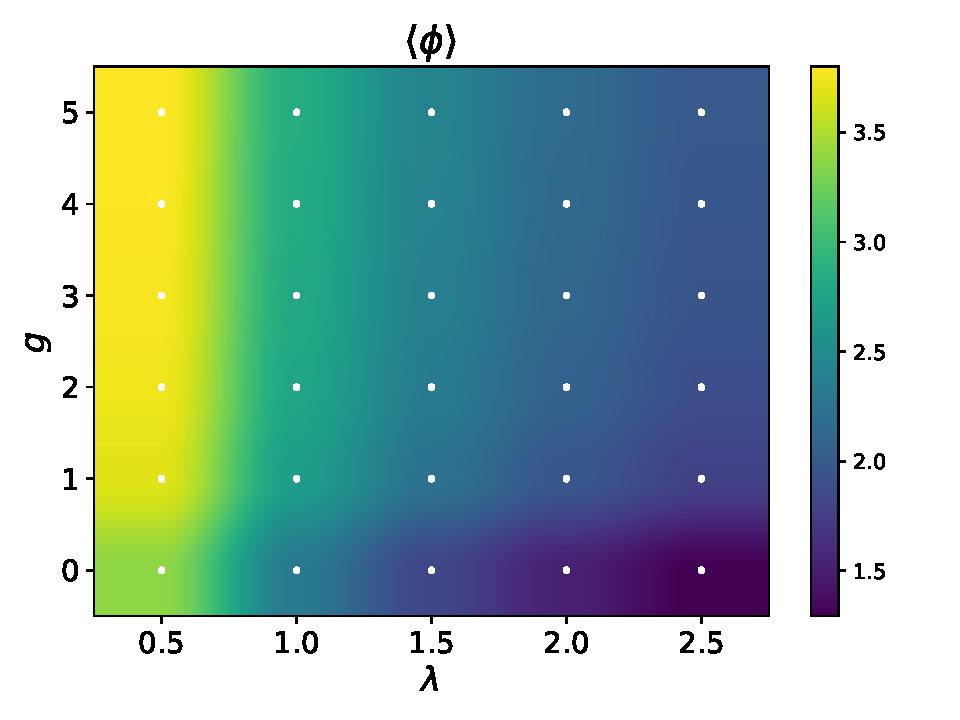
\includegraphics[width=\textwidth]{figures/phase_diagram/g-lam/phase_diagram_phi.pdf}
    \end{subfigure}
    \begin{subfigure}[b]{0.47\textwidth}
        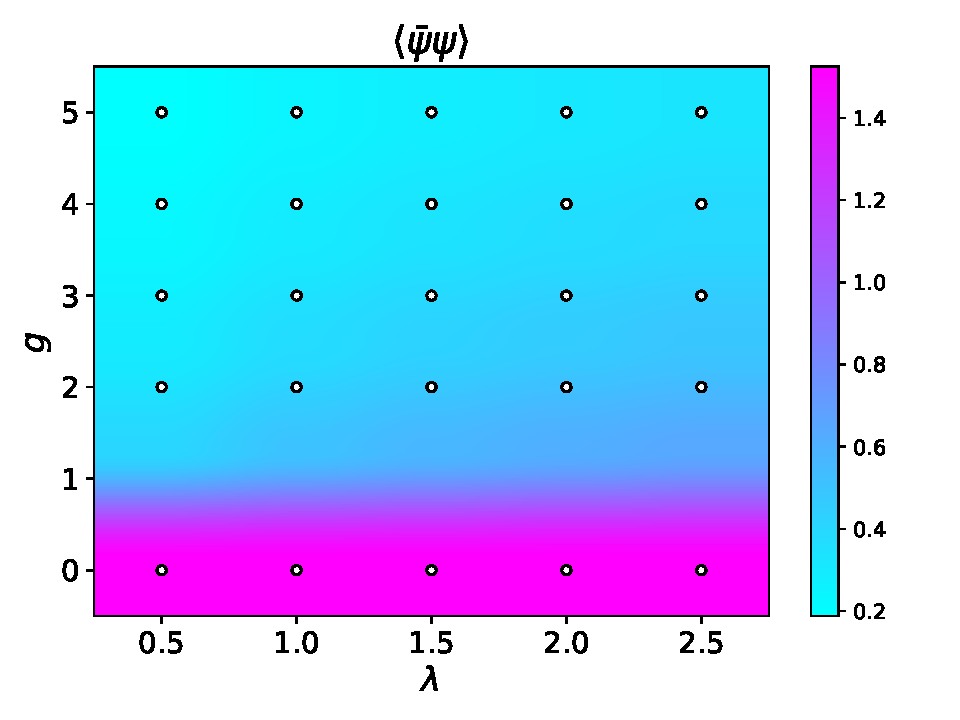
\includegraphics[width=\textwidth]{figures/phase_diagram/g-lam/phase_diagram_cond.pdf}
    \end{subfigure}
    \begin{subfigure}[b]{0.47\textwidth}
        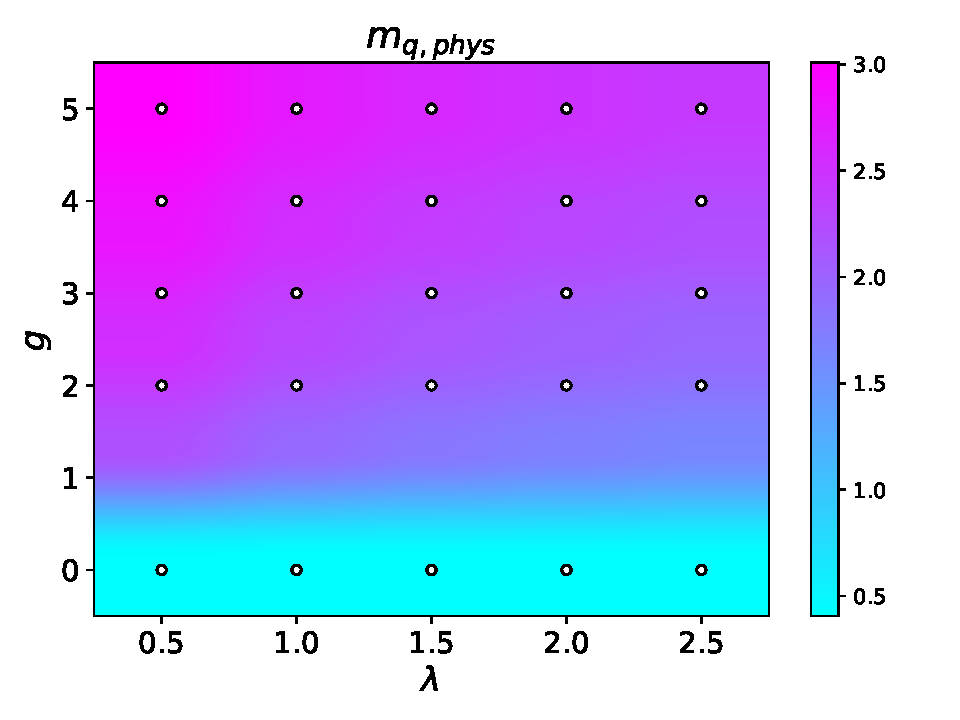
\includegraphics[width=\textwidth]{figures/phase_diagram/g-lam/phase_diagram_mqphys.pdf}
    \end{subfigure}
    \begin{subfigure}[b]{0.47\textwidth}
        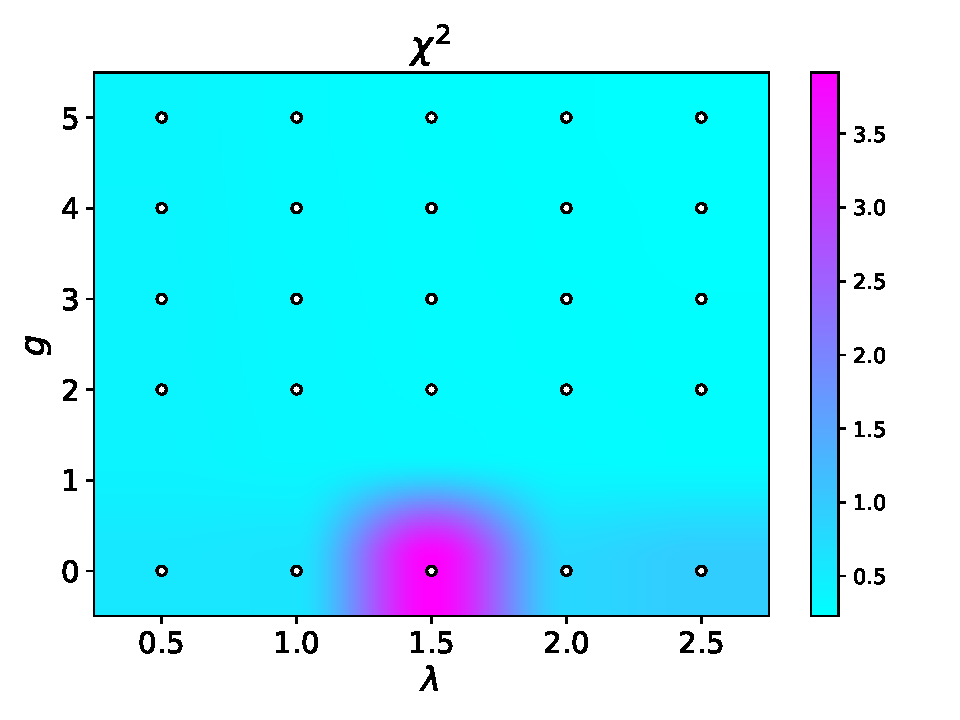
\includegraphics[width=\textwidth]{figures/phase_diagram/g-lam/phase_diagram_chi2.pdf}
    \end{subfigure}
    \caption{Slice of the phase diagram at fixed $m_\phi^2 = -1.0$. \\ Lattice size $32 \times 32$, $N_\text{conf} \approx \mathcal{O}(10^4)$.}
    \label{fig:phase_diagram_g_lam}
\end{figure} \newpage
Finally, let us give a look at the phase structure in the $\lambda - m_\phi^2$ plane. 
Since here one always has $g \neq 0$, the expectation value of the scalar field and the chiral condensate are never zero, since the symmetry is broken independetly of the choice of $m_\phi^2$ and $\lambda$. This fact is also reflected in the mass plot,
where one can clearly see that $m_{q,\text{phys}}$ is always proportional to the field.
\begin{figure}[hbp]
    \centering
    \begin{subfigure}[b]{0.47\textwidth}
        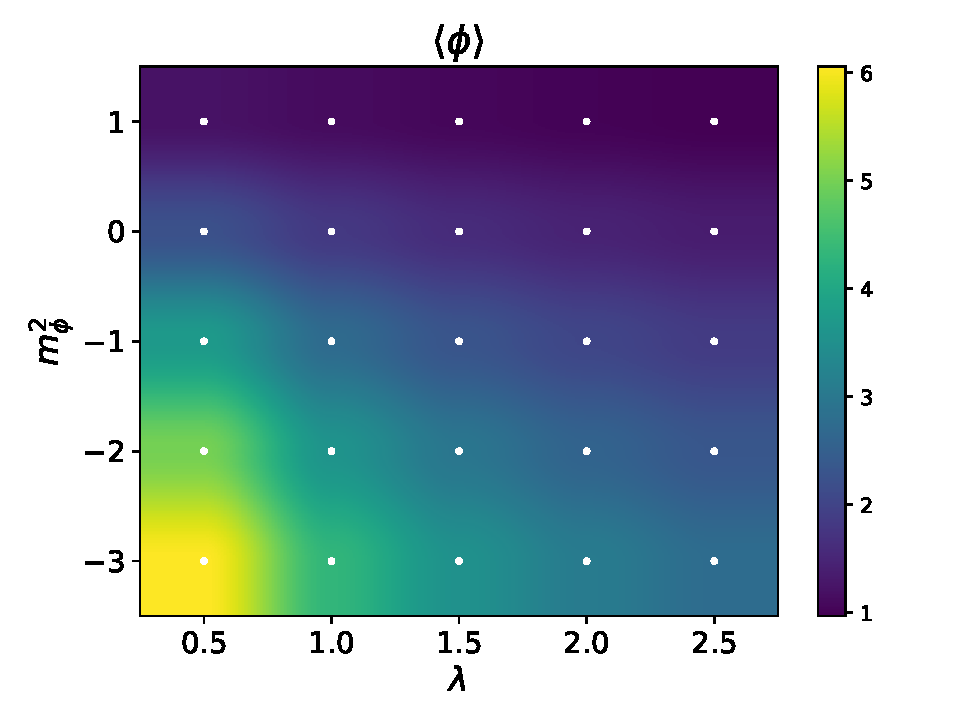
\includegraphics[width=\textwidth]{figures/phase_diagram/m-lam/phase_diagram_phi.pdf}
    \end{subfigure}
    \begin{subfigure}[b]{0.47\textwidth}
        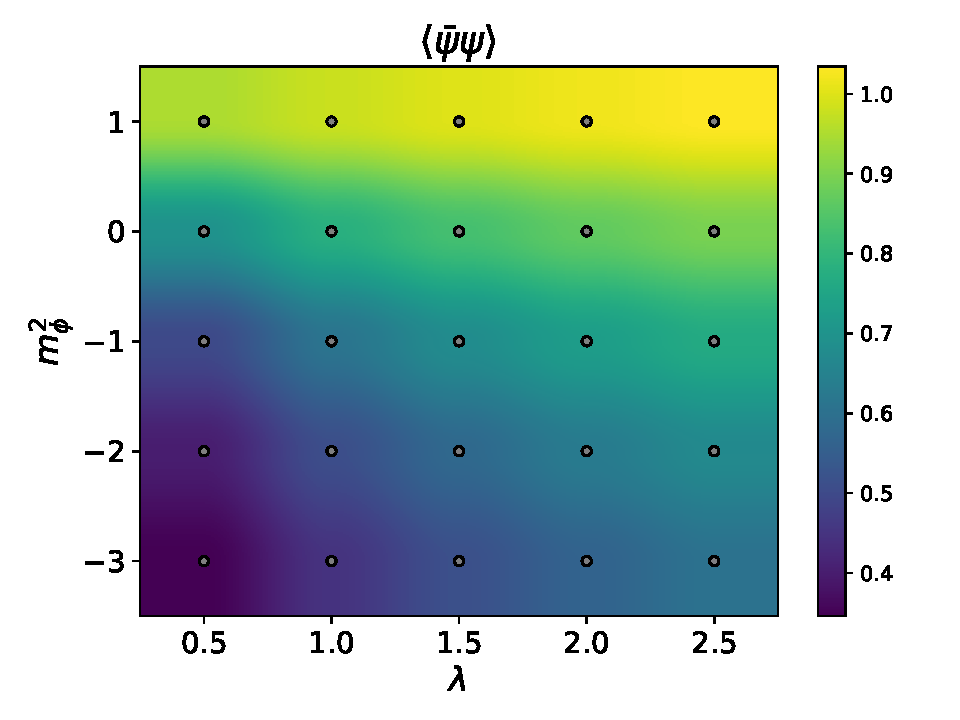
\includegraphics[width=\textwidth]{figures/phase_diagram/m-lam/phase_diagram_cond.pdf}
    \end{subfigure}
    \begin{subfigure}[b]{0.47\textwidth}
        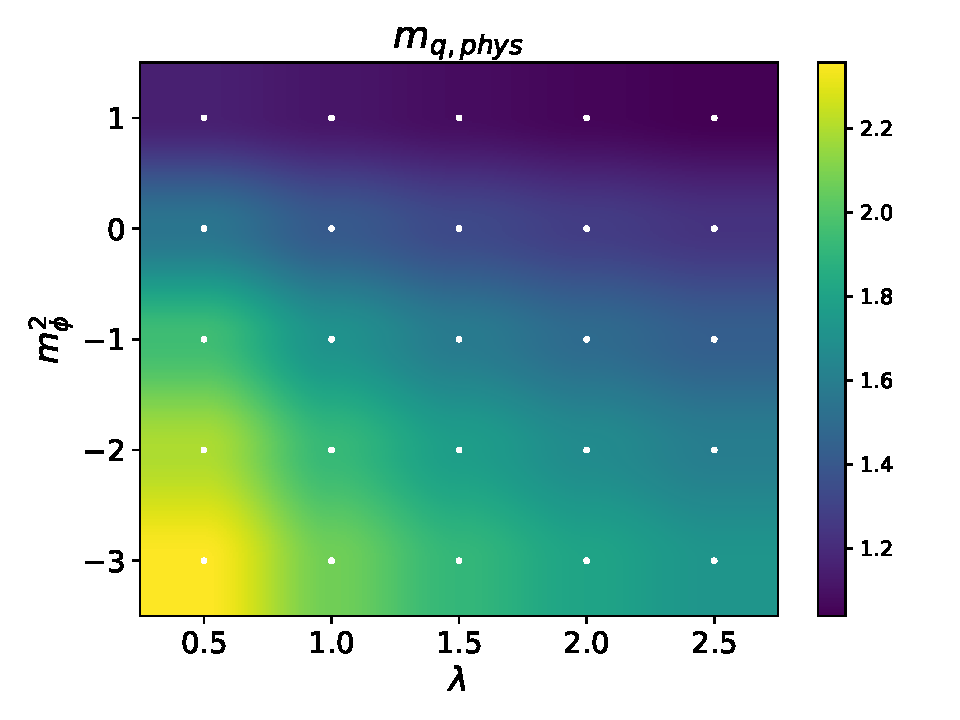
\includegraphics[width=\textwidth]{figures/phase_diagram/m-lam/phase_diagram_mqphys.pdf}
    \end{subfigure}
    \begin{subfigure}[b]{0.47\textwidth}
        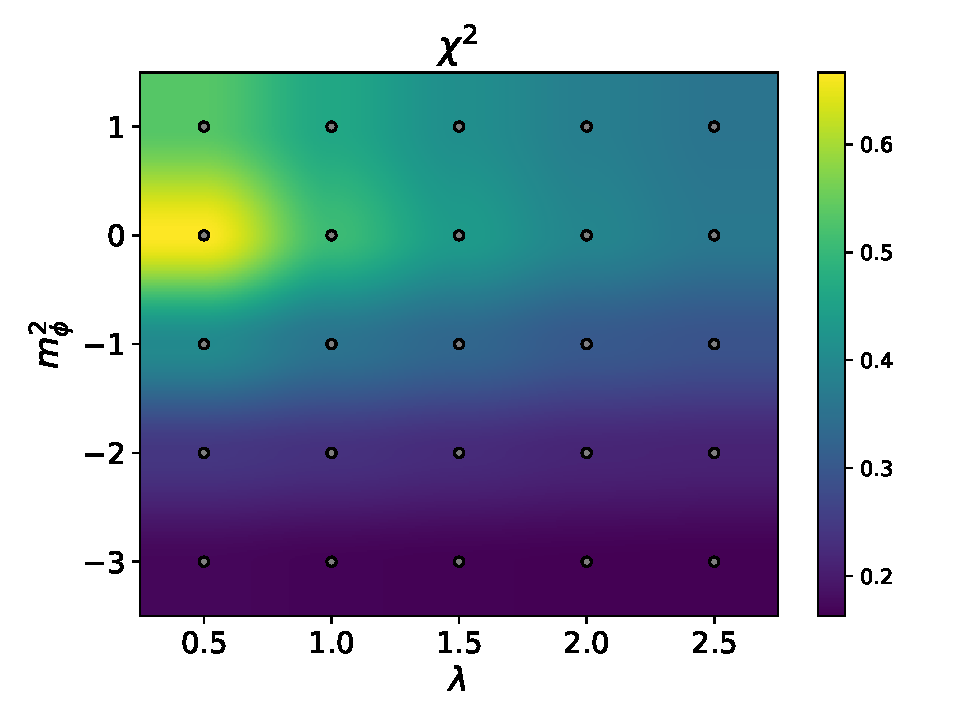
\includegraphics[width=\textwidth]{figures/phase_diagram/m-lam/phase_diagram_chi2.pdf}
    \end{subfigure}
    \caption{Slice of the phase diagram at fixed $g = 1.5$. \\ Lattice size $64 \times 64$, $N_\text{conf} \approx \mathcal{O}(10^4)$.}
    \label{fig:phase_diagram_m_lam}
\end{figure}\\
Moreover, the susceptibility in this case does not show a single peak as the phase transition can only happen for $g=0$. Note in fact the difference in magnitude with respect to figures \ref{fig:phase_diagram_g_m} and \ref{fig:phase_diagram_g_lam}.

\chapter{Numerical investigation: coloured noise}
\label{chapt:results_coloured}

\section{Classical-to-quantum interpolation}
\label{sec:classical_to_quantum}
\begin{figure}[h]
    \centering
    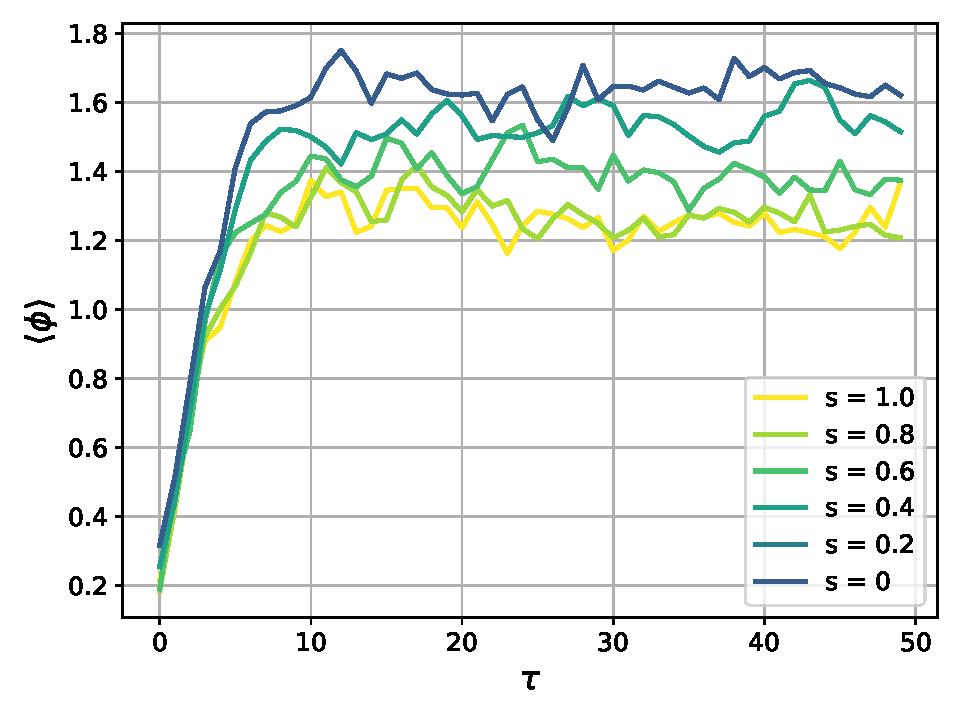
\includegraphics[width=0.8\textwidth]{figures/slide_broken/thermalisation.pdf}
    \caption[Thermalisation of the system for different values of the noise fraction $s$.]{Thermalisation of the system for different values of the noise fraction $s$. As noise is added, the equilibrium state of the system shifts accordingly. Coloured noise allows for a smooth interpolation between the fully classical and fully quantum picture.\\ Lattice size $32 \times 32, \ m_\phi^2=-1.0, \ \lambda=0.5, \ g=0.08, \ m_q = 0.5$.}
    \label{fig:thermalisation_different_noise_fracs}
\end{figure}
Let us start by analising the coloured noise field in the simulation and relevant properties that emerge from it. We consider the Yukawa model described by the continuum action \eqref{eq:full_action_continuum} and its discrete version \eqref{eq:discretised_action}, \eqref{eq:discretised_effective_action}.\\
The system is initialised in the same state for all the configurations on a $64 \times 64$ lattice. We consider a simulation with $s=1$ and then progressively lower the cutoff fraction $s$, keeping fixed all the quantities in the classical action. \\
Figure \ref{fig:thermalisation_different_noise_fracs} shows the system thermalisation for different values of $s$, namely the Langevin evolution from the initial state to equilibrium. The blue line corresponds to the case $s=0$, a classical simulation, while the yellow line corresponds to the $s=1$, the fully quantum case.  All the parameters settings are reported under the figure. As quantum modes are removed via coloured noise, the system shifts its equilibrium point. \\~\\ 
We now want to make use of coloured noise to understand the relation between scalar field, quark condensate and fermionic mass, which was qualitatively discussed in section \ref{sec:Yukawa_theory} by means of classical arguments. \\
Keeping all the parameters fixed, we perform simulations changing the value of the cutoff fraction $s$, and we measure the three quantities above mentioned: the results are reported in figure \ref{fig:interpolation_relation_phi_cond_mass}. 
One can clearly see that as quantum modes are added, one has
\begin{equation*}
	\expect{\phi} \sim \expect{\bar\psi\psi} \sim m_q.
\end{equation*}
\begin{figure}[h]
    \centering
    \begin{subfigure}[b]{0.47\textwidth}
        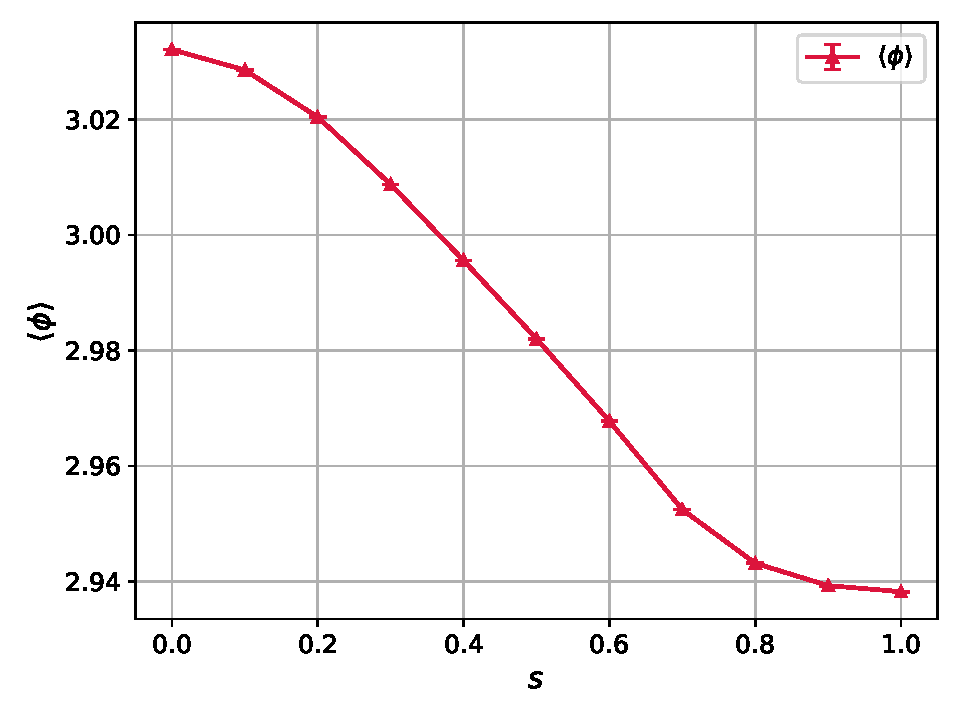
\includegraphics[width=1.0\textwidth]{figures/slide_broken/magnetisation.pdf}
        \caption{Magnetisation}
    \end{subfigure}
    \begin{subfigure}[b]{0.47\textwidth}
        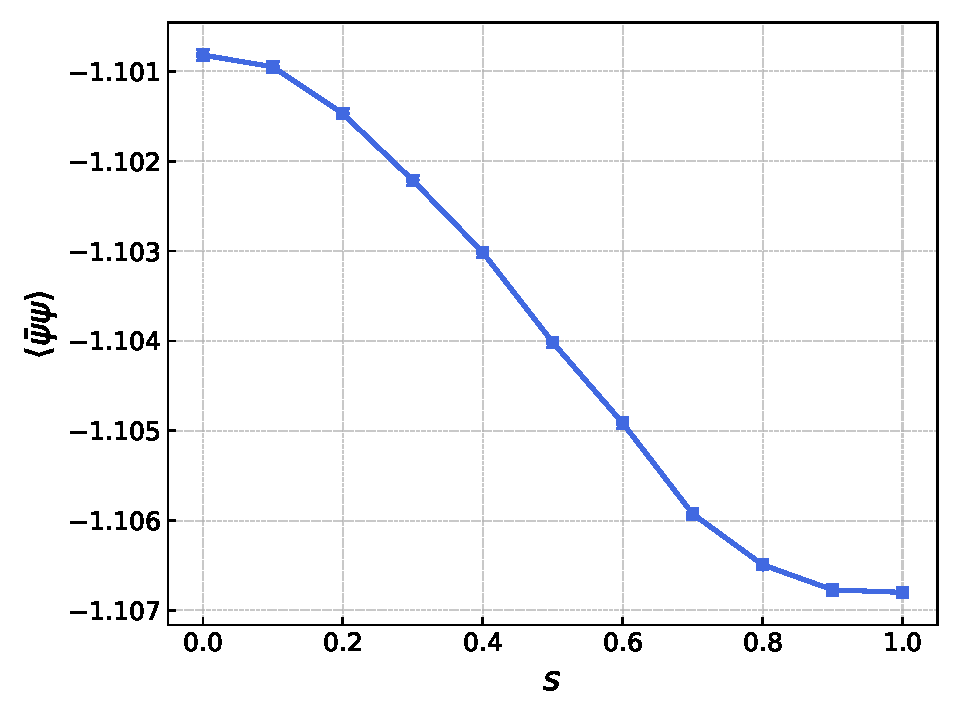
\includegraphics[width=1.0\textwidth]{figures/slide_broken/condensate.pdf}
        \caption{Chiral condensate}
    \end{subfigure}
    \begin{subfigure}[b]{0.47\textwidth}
        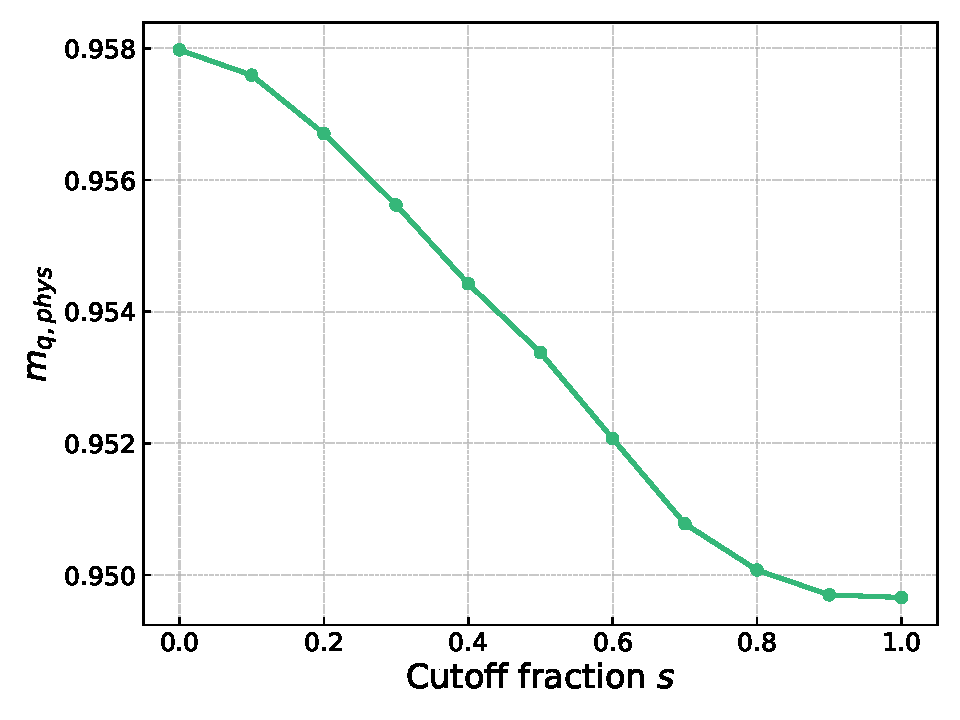
\includegraphics[width=1.0\textwidth]{figures/slide_broken/mass.pdf}
        \caption{Physical quark mass}
    \end{subfigure}
    \caption[Relation between magnetisation, condensate and mass]{Relation between magnetisation, chiral condensate and mass, which was motivated in section \ref{sec:Yukawa_theory}. \\ $m_\phi^2=-1.0, \ \lambda=0.7, g=0.2, \ m_q = 1.0$ \\ Lattice size $64 \times 64, \ N_\text{conf} \approx \mathcal{O}(5 \cdot 10^4)$.}
    \label{fig:interpolation_relation_phi_cond_mass}
\end{figure} \\
This makes clear at first that the scalar field $\phi$ effectively plays the role of quark bilinear in the dynamics. Moreover, the physical mass of the quark grows proportionally to the scalar field magnetisation at all levels in the quantum theory. \\
The interconnection of these phenomena is an important result if one interprets it in the context of effective theories. In fact, often in QCD, the dynamical chiral symmetry breaking mechanism is described by low energy Yukawa-type effective models such as Gross-Neveu, Nambu - Jona-Lasinio or Quark Meson, to name some examples, where a scalar field can emerge after bosonisation via a Hubbard-Stratonovich transformation \textcolor{red}{cite}. \\
Independetly of this, studying the behavior of observables as a function of the cutoff fraction $s$, allows to understand better the role of fluctuations in the system and which degrees of freedom give more contribution to the dynamics.
\section{Chiral fermions and noise-induced transition}
\label{sec:chiral_PT}
As explained in section \ref{sec:Yukawa_theory}, chiral symmetry can be broken, in the continumm theory, either explicitly via the introduction of a finite bare quark mass, or spontaneously if the field gains a non-zero expectation value.\\
Moreoveor, in the discrete formulation, the introduction of the Wilson term contributes to the explicit breaking of chiral symmetry, as shown in appendix \ref{chap:AppendixB}. This, in particular, means that chiral symmetry is explicitly broken also for $m_q \to 0$. Because of this, one needs a new definition of the bare mass $M_q$, which takes into account the Wilson term contribution, such that chiral symmetry is restored in the limit $M_q \to 0$. \\
In a lattice study of a theory suchs as  two-flavours QCD, what one typically does \cite{rothe_LGT,gattringer_LQCD} is the following: the spontaneous breaking of chiral symmetry generates three goldstone massless bosons, the pions. If the bare quark mass is zero, the physical mass of the pions has to be zero, as a consequence of Goldstone's theorem \cite{goldstone}. Hence one can measure the pions mass and find a value $m_q^*$ such that when $m_q \to m_q^*$, one has $m_\pi \to 0$. \\
This approach is not feasible in our theory, since it is described by a discrete chiral symmetry, and no Goldstone modes appear as a consequence. A possible way of proceeding \cite{Bermudez2018} could be to tune the bare quark mass as a function of the interaction couplings in order to set the renormalised mass to zero, causing the divergence of a correlation length. In this case, the physical quantities of interest become independent of
the underlying lattice, and one expects to recover the desired continuum QFT. A discussion on the issue, together with other proposals for the definition of the bare quark mass for similare theories can be found in \cite{Iwasaki:1994gq,MAIANI1986265}. We do not follow such approaches here, mostly because of time limits, but also because it is not our purpose to match any precise model, but rather investigate properties of the coloured noise technique. In this section we just consider na\"ive fermions and the chiral limit is reached for $m_q \to 0$. Thus, one has to keep in mind that due to the fermion doubling this represents a theory with $2N_f = 4$ degenerate quarks.
\begin{figure}[h]
    \centering
    \captionsetup[subfigure]{justification=centering}
    \begin{subfigure}[t]{0.47\textwidth}
        \centering
        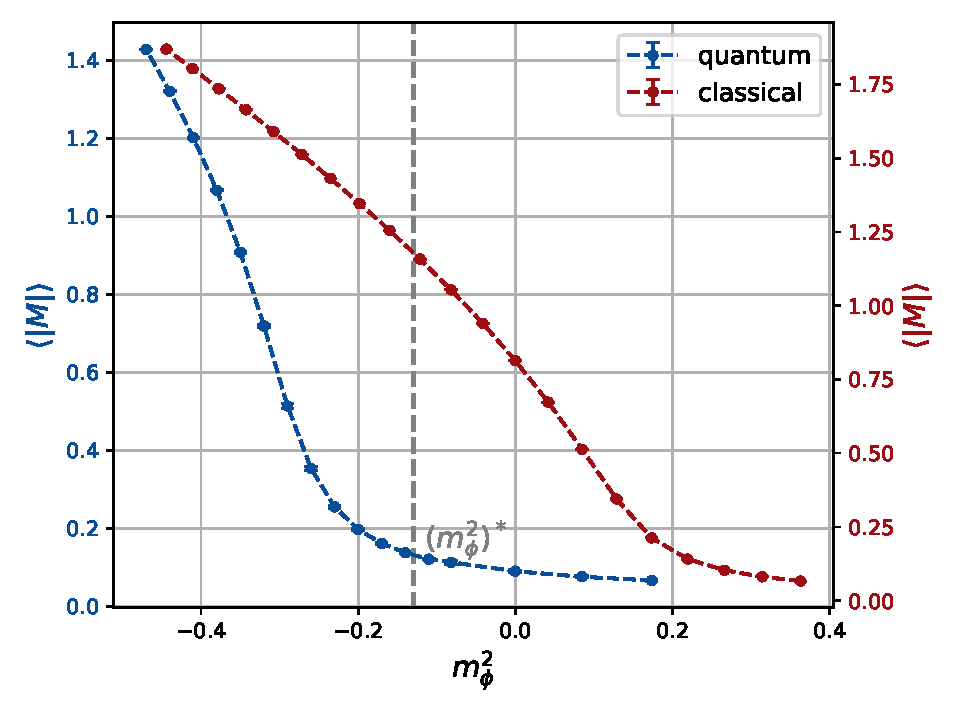
\includegraphics[width=1.0\textwidth]{figures/chiral_PT/mass_scan/magnetisation.pdf}
        \caption{Magnetisation}
    \end{subfigure}
    \hfill
    \begin{subfigure}[t]{0.47\textwidth}
        \centering
        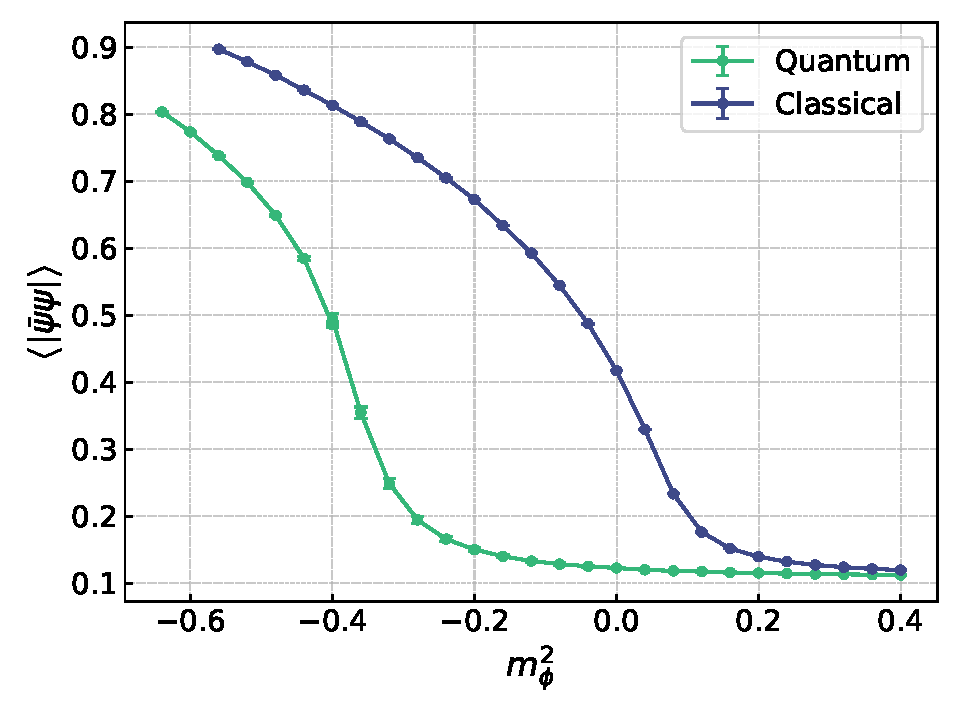
\includegraphics[width=1.0\textwidth]{figures/chiral_PT/mass_scan/condensate.pdf}
        \caption{Chiral condensate}
    \end{subfigure}
    \caption[Scalar mass scan of the quantum and classical theories]{Scalar mass scan of the quantum and classical theories. \\ One can see that for values of scalar squared mass $-0.2 \leq m_\phi^2 \leq 0$, the classical and the quantum systems lie in two different phases. \\
    $\lambda=1.951, g=0.08,$ Lattice size $32 \times 32, \ N_\text{conf} \approx \mathcal{O}(10^4)$}
    \label{fig:scans_classical_quantum}
\end{figure} \\
In figure \ref{fig:scans_classical_quantum}, the (absolute) magnetisation and the chiral condensate are studied as a function of the bosonic mass squared, both in the fully quantum and fully classical theory. One can notice that the classical system undergoes a phase transition at values of $m_\phi^2$ bigger than the quantum counterpart. \\
Note that as the bare quark mass is small but finite, this is not a proper phase transition and the latter will be, eventually, reached in the limit $m_q \to 0$. \\
We then pick a value $m_\phi^{2 \, *} = -0.123$. Using coloured noise, we then interpolate between the classical and quantum picture for different values of the quark mass, namely $m_q = 10^{-2}, \, 5 \cdot 10^{-3}, \, 10^{-3}$.
\begin{figure}[h!]
\centering
\begin{subfigure}{0.47\textwidth}	
	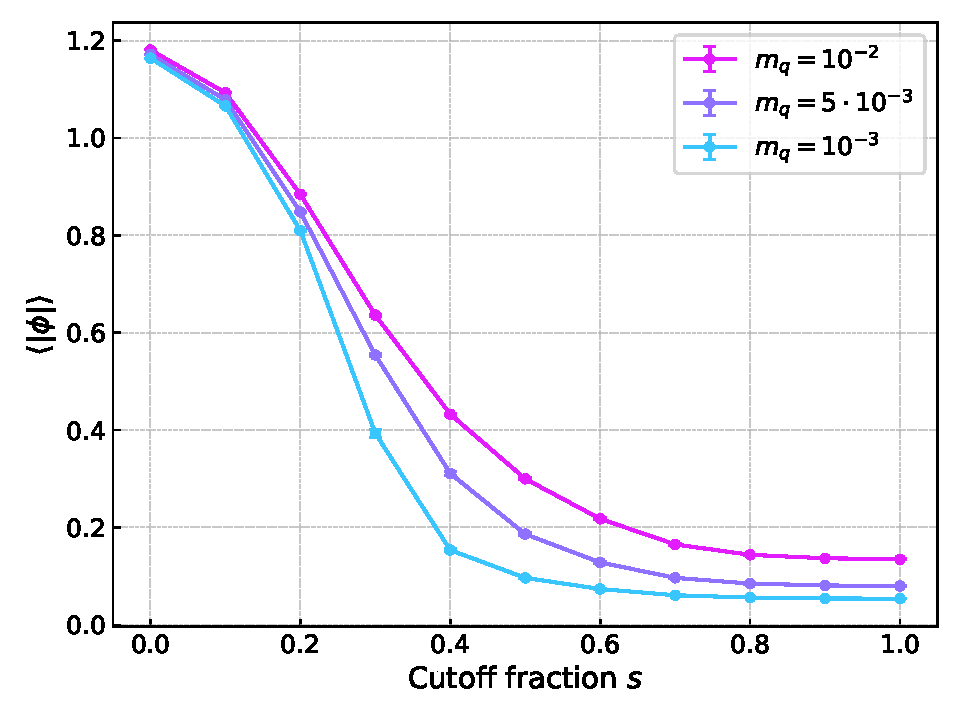
\includegraphics[width=\textwidth]{figures/chiral_PT/magnetisation.pdf}
    \caption{Magnetisation}
\end{subfigure}
\begin{subfigure}{0.47\textwidth}	
	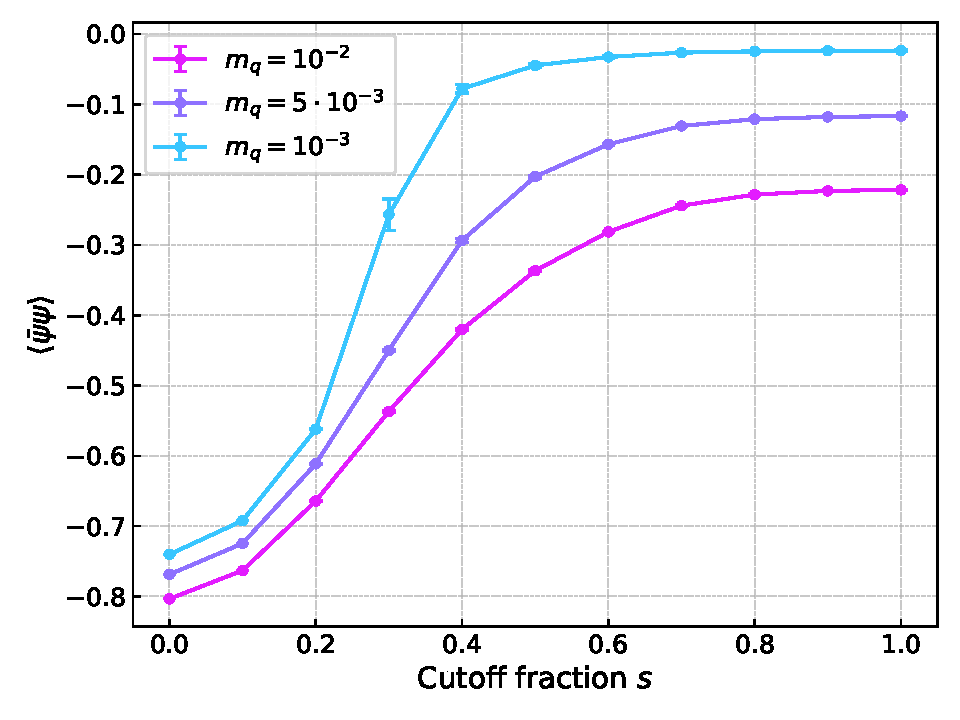
\includegraphics[width=\textwidth]{figures/chiral_PT/condensate.pdf}
    \caption{Chiral condensate}
\end{subfigure}
\begin{subfigure}{0.47\textwidth}	
	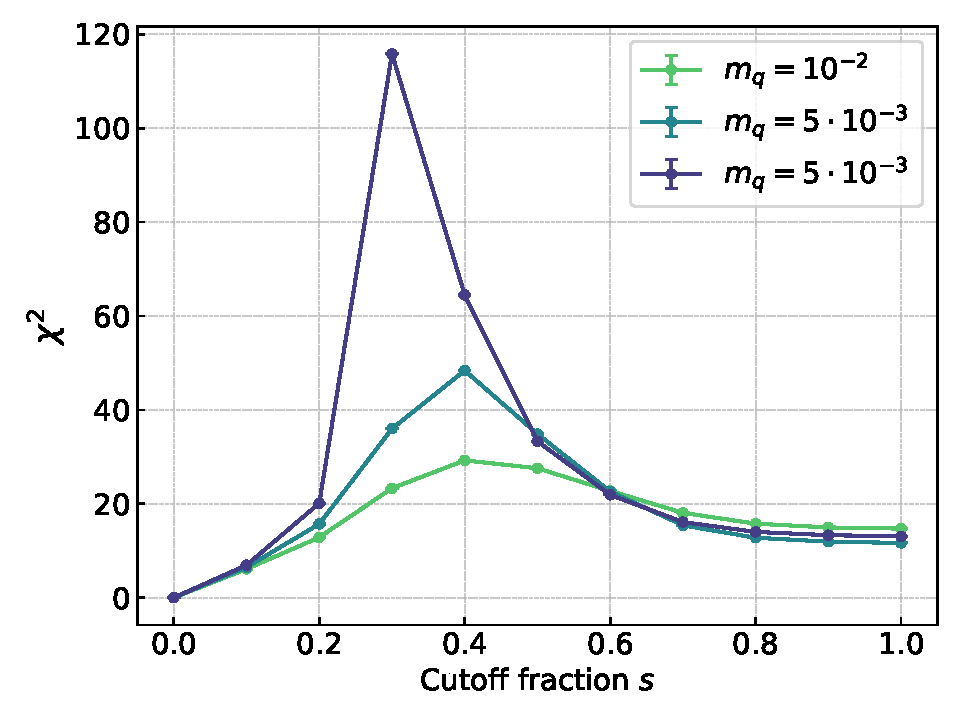
\includegraphics[width=\textwidth]{figures/chiral_PT/chi2.pdf}
    \caption{Susceptibility}
\end{subfigure}
\begin{subfigure}{0.47\textwidth}
	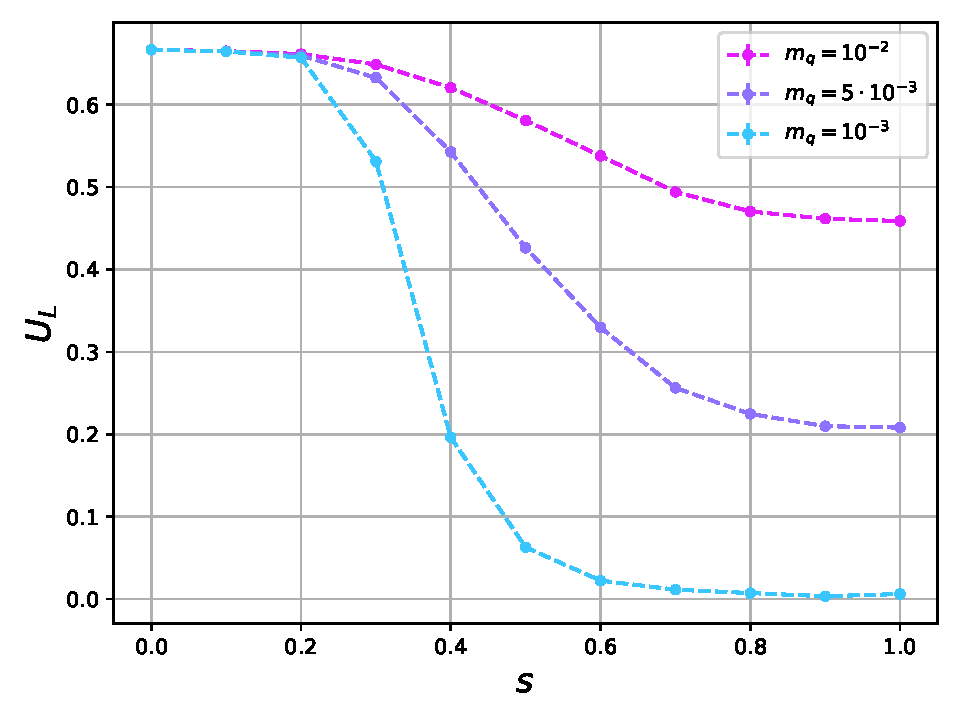
\includegraphics[width=\textwidth]{figures/chiral_PT/binder.pdf}
    \caption{Binder cumulant}
\end{subfigure}\\
\begin{subfigure}{0.47\textwidth}
    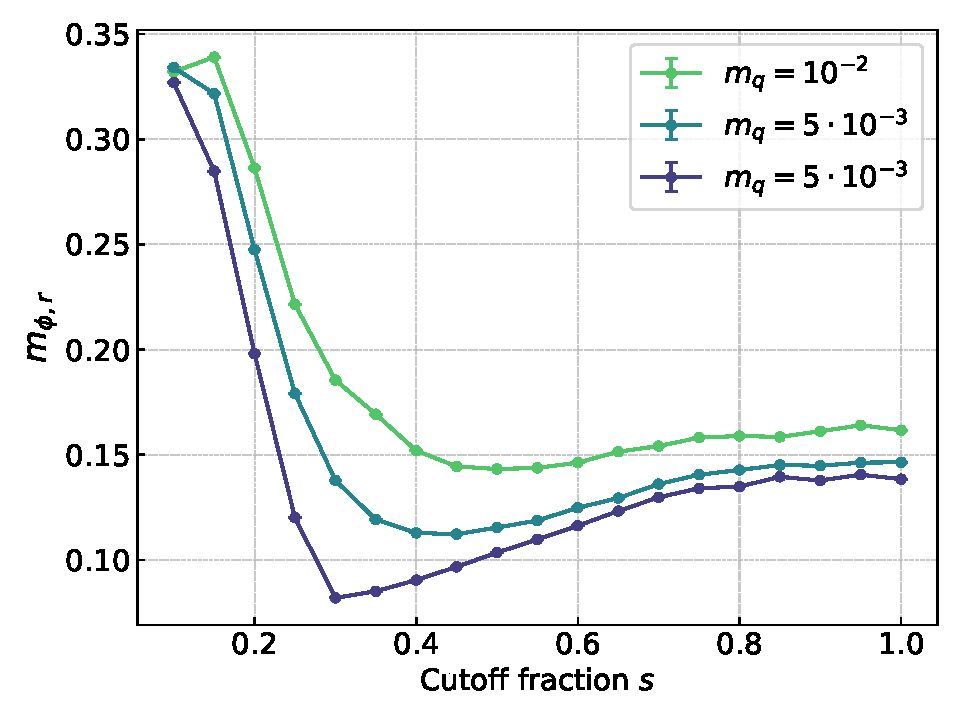
\includegraphics[width=\textwidth]{figures/chiral_PT/mphir.pdf}
    \caption{Renormalised scalar mass}
\end{subfigure}
\caption{$m_\phi^2=-0.123, \ \lambda=1.951, g=0.08,$ \\ Lattice size $64 \times 64, \ N_\text{conf} \approx \mathcal{O}(5 \cdot 10^4)$}
\label{fig:chiral:symmetry_breaking}
\end{figure}\\
One can clearly see in figure \ref{fig:chiral:symmetry_breaking} that as the quark  mass is lowered the difference between the two phases gets more pronounced, indicating a phase transition. \\
Both the magnetisation and the chiral condensate are finite in the classical theory and get washed out as quantum fluctuations are added. 
The peak in the susceptibility shows the transition is happening for $0.2 \leq s \leq 0.4$, but the resolution is not enough to determine the precise value of $s$. \\ 
The Binder parameters assumes the value $U_L = 0$ in the symmetric phase, and $U_L=2/3$ in the broken phase, as expected. Finally, the scalar renormalised mass tends to zero as the transition point is approached, signaling the divergence of the correlatin length. \\
Hence all the five observables are in agreement and signal the presence of a phase transition. \\
Intuitively speaking one can interpret the situation by looking at figure \ref{fig:breaking_O1_symmetry}. For $m_\phi^2 < 0$, the classical potential has two minima that are slightly inequivalent 
due to the presence of a small yukawa coupling. In the classical theory, the system is constrained at the global minimum, since there is no stochasticity and the kinetic term is not strong enough to cause the hopping between the two minima. At the quantum level, fluctuations allow such transition bringing $\expect{\phi} \to 0$ and restoring the symmetry.
Note that in order to confirm that a phase transition took place, one should first consider $V \to \infty$ and then $m_q \to 0$. If the order parameters of the classical and quantum theories still indicates that the system is 
in two different phases, one can draw the conclusion. \\~\\
In this context, it would be interesting to look at the physical quark mass. In fact, neglecting the bare quark mass $m_q \approx 0$, one would expect the fermions to be massive in the classical theory due to the presence of the background field $\phi$, which work as an additional mass. In the classical-to-quantum transition, as the field expectation vanishes, the 
fermions become massless. Thus, due to the choice of discretisation, namely employing naive fermions, it is not possible to extract the quark mass in a straightforward way due to the proprties of the doublers. The latter exhibits in fact an incorrect momentum dispersion relation \cite{COHEN1983102,PhysRevD.101.094512}. \textcolor{blue}{we thought it was the choice of the source but it is not. I might try to add an appendix in which I show the plot of what happens there.}

\newpage

\section{Cooling with coloured noise}
Let us now consider one of the main applications of coloured noise, namely the cooling technique. \\
We first set up a white noise simulation $s=1$, and then progressively lower $s$. The lowering of the cutoff is compensated by a change in the couplings, as explained in section \ref{sec:lattice_with_coloured_noise}. 
We study the behavior of the system both as a function of the bosonic mass squared $m_\phi^2$ and the Yukawa coupling $g$. 
A summary of the parameters choice for both the experiments is reported in tables \ref{tab:params_cooling} and \ref{tab:params_cooling_yukawa}.
\begin{table}[htp]
    \centering
    \begin{tabular}{cccccccc}
        \toprule
        $s$ & $N_t$ & $N_x$ & $m_\phi^2$ & $\lambda$ & $g$ & $m_q$& $K_\psi$ \\
        \midrule 
        1 & 16 & 16 & $m_\phi^2$ & 0.4 & 0.3 & $0.5$ & $K_\psi$ \\
        1/2 & 32 & 32 & $m_\phi^2/4$ & 0.1 & 0.3 & $0.5$ & $K_\psi/4$ \\
        1/4 & 64 & 64 & $m_\phi^2/16$ & 0.025 & 0.3 & $0.5$ & $K_\psi/16$ \\
        1/8 & 128 & 128 & $m_\phi^2/64$ & 0.00625 & 0.3 & $0.5$ & $K_\psi/64$ \\
        \bottomrule
    \end{tabular}
    \caption[Parameter settings in the cooling procedure for the Bosonic mass squared scan]{Parameter settings in the cooling procedure for the bosonic mass squared scan. Each coupling in the bosonic action is rescaled according to its canonical dimension, while the fermionic sector rescaling is implemented directly at the drift level, as detailed in section \ref{sec:lattice_with_coloured_noise}}.
    \label{tab:params_cooling}
\end{table}
\begin{table}[htp]
    \centering
    \begin{tabular}{cccccccc}
        \toprule
        $s$ & $N_t$ & $N_x$ & $m_\phi^2$ & $\lambda$ & $g$ & $m_q$& $K_\psi$ \\
        \midrule 
        1 & 16 & 16 & $0.5$ & 0.7 & g & $1.0$ & $K_\psi$ \\
        1/2 & 32 & 32 & $0.125$ & 0.175 & g & $1.0$ & $K_\psi/4$ \\
        1/4 & 64 & 64 & $0.0625$ & 0.04375 & g & $1.0$ & $K_\psi/16$ \\
        1/8 & 128 & 128 & $0.03125$ & 0.001094 & g & $1.0$ & $K_\psi/64$ \\
        \bottomrule
    \end{tabular}
    \caption[Parameter settings in the cooling procedure for the Yukawa coupling scan.]{Parameters setting in the cooling procedure for the Yukawa coupling scan. Each coupling in the bosonic action is rescaled according to its canonical dimension, while the fermionic sector rescaling is implemented directly at the drift level, as detailed in section \ref{sec:lattice_with_coloured_noise}}.
    \label{tab:params_cooling_yukawa}
\end{table} \\
Figure \ref{fig:cooling_M_psibarpsi_chi2} reports the magnetisation, its susceptibility and the chiral condensate as a function of the bare scalar mass squared $m_\phi^2$, while figure \ref{fig:cooling_M_psibarpsi} reports the investigation as a function of the Yukawa coupling.
One can clearly see that there is a general good agreement for the first three block-spin transformations, even if based on tree level arguments.
\begin{figure}[hbp]
    \centering
    \begin{subfigure}[b]{0.47\textwidth}
        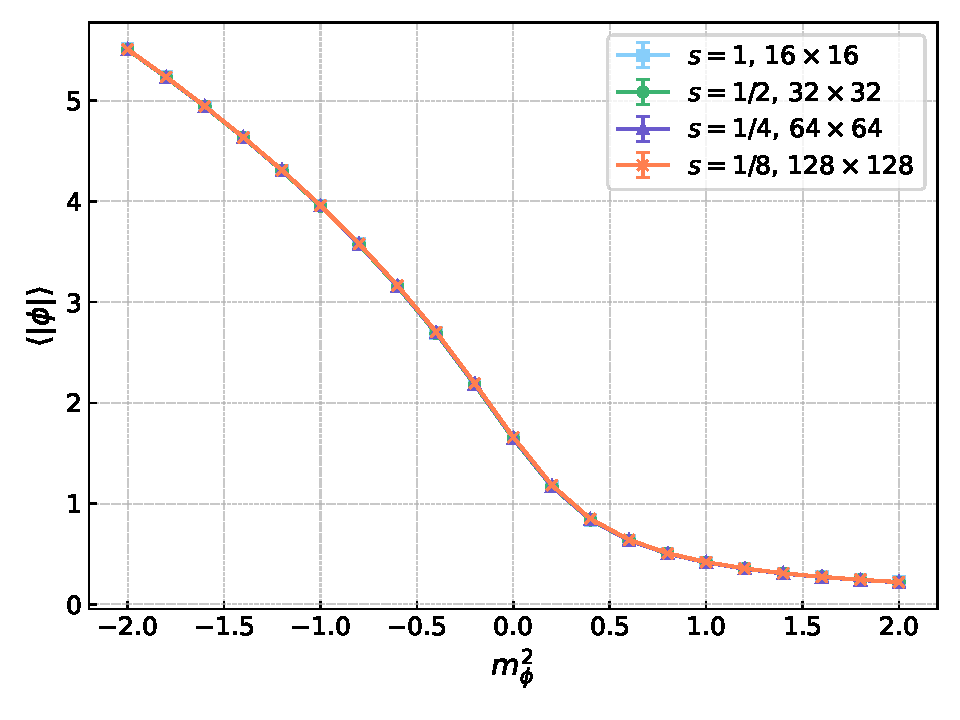
\includegraphics[width=\textwidth]{figures/cooling/mass_scan/magnetisation.pdf}
        \caption{Magnetisation}
    \end{subfigure}
    \hfill
    \begin{subfigure}[b]{0.47\textwidth}
        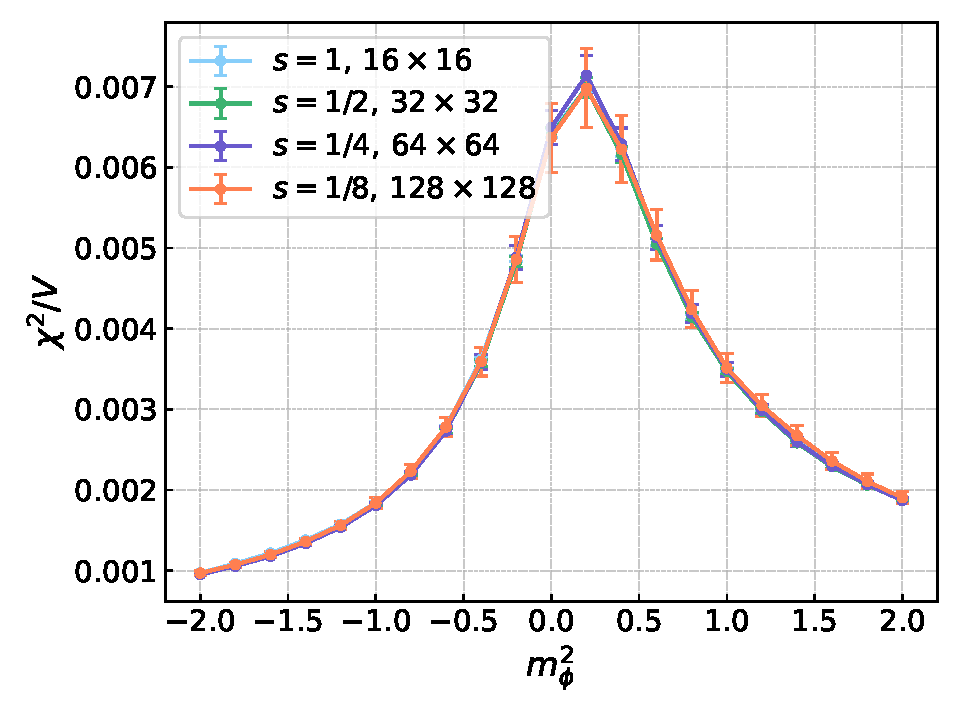
\includegraphics[width=\textwidth]{figures/cooling/mass_scan/susceptibility.pdf}
        \caption{Susceptibility}
    \end{subfigure}
    \begin{subfigure}[b]{0.47\textwidth}
        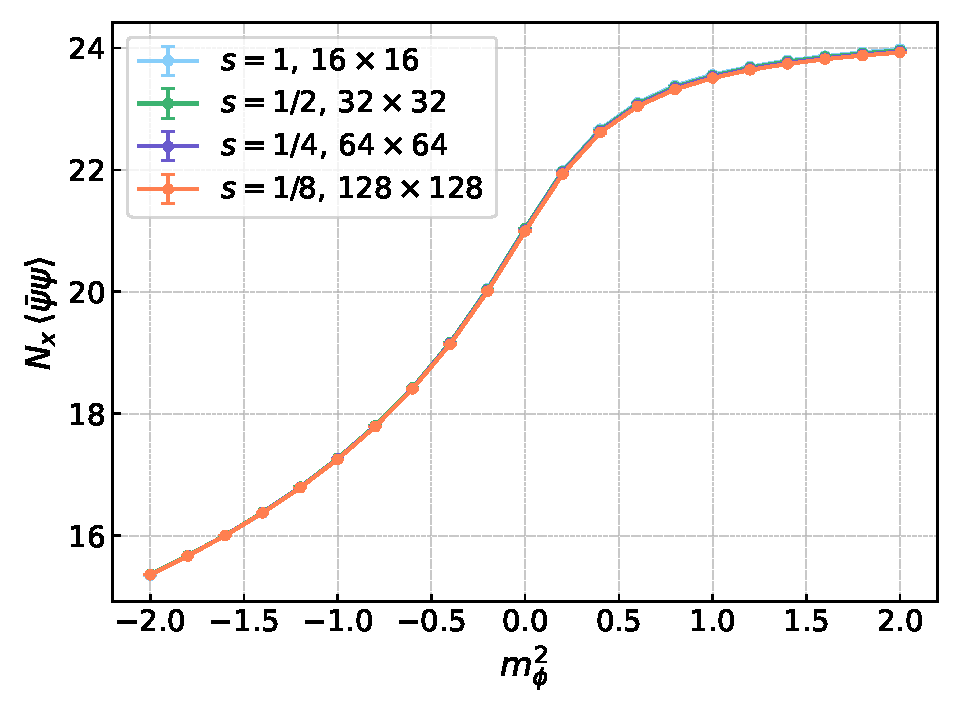
\includegraphics[width=\textwidth]{figures/cooling/mass_scan/condensate.pdf}
        \caption{Chiral condensate}
    \end{subfigure}
    \caption[Cooling stochastic quantisation: fields as a function of the bosonic mass squared.]{Cooling via coloured noise. The absolute magnetisation, its susceptibility and the chiral condensate are compared after performing block-spins transformations as a function of the bosonic mass squared. All the parameters are reported in table \ref{tab:params_cooling}. \\ $N_\text{conf} \approx \mathcal{O}(5 \cdot 10^4)$.}
    \label{fig:cooling_M_psibarpsi_chi2}
\end{figure}
\begin{figure}[hbp]
    \centering
    \begin{subfigure}[b]{0.47\textwidth}
        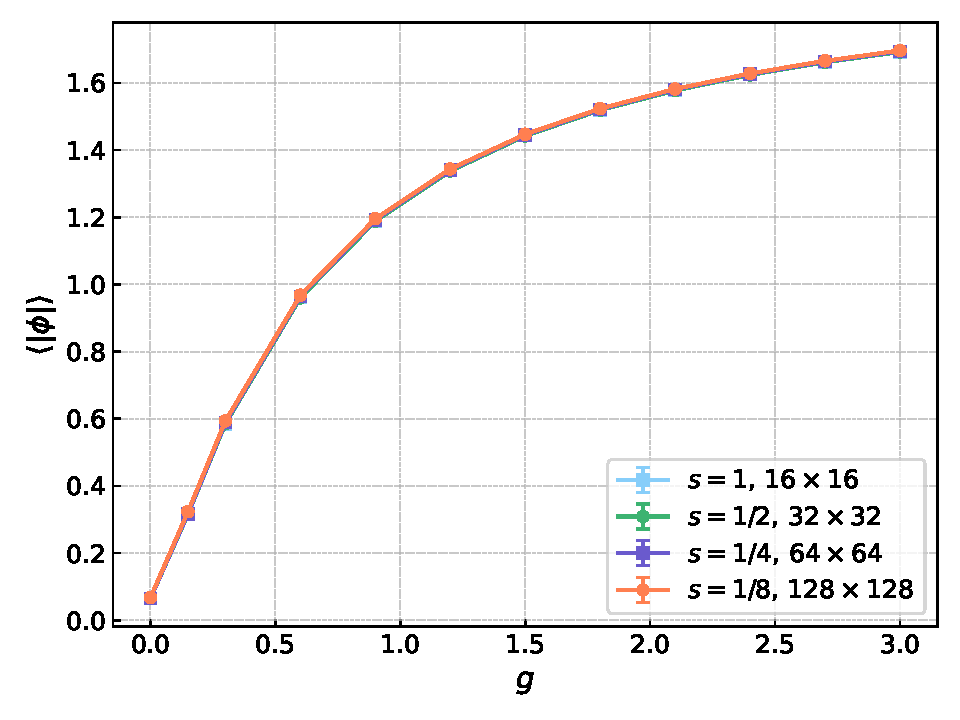
\includegraphics[width=\textwidth]{figures/cooling/yukawa_scan/magnetisation.pdf}
        \caption{Magnetisation}
    \end{subfigure}
    \hfill
    \begin{subfigure}[b]{0.47\textwidth}
        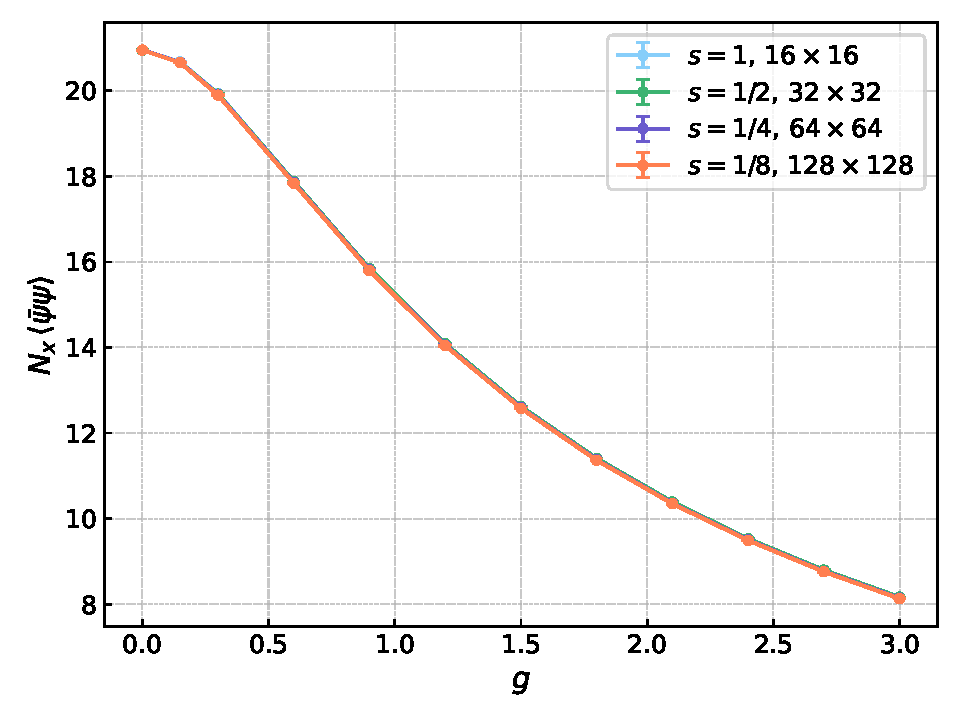
\includegraphics[width=\textwidth]{figures/cooling/yukawa_scan/condensate.pdf}
        \caption{Chiral condensate}
    \end{subfigure}
    \caption[Cooling stochastic quantisation: fields as a function of the Yukawa coupling.]{Cooling via coloured noise. The absolute magnetisation and the chiral condensate are compared after performing block-spins transformations as a function of the Yukawa coupling. \\ All the parameters are reported in table \ref{tab:params_cooling_yukawa}. \\$N_\text{conf} \approx \mathcal{O}(5 \cdot 10^4)$. }
    \label{fig:cooling_M_psibarpsi}
\end{figure}
\newpage
The most relevant observables are the magnetisation and the chiral condensate, since they are the order parameters of the theory. We therefore want to provide a more detailed comparison of the performance of the procedure. To this end we define the relative errors
\begin{equation}
    \begin{aligned}
        \epsilon_\phi(s) &= \frac{\expect{|M|}_{s} - \expect{|M|}}{\expect{|M|}}, \\
        \epsilon_\psi(s) &= \frac{N_x^{(s)} \,\expect{|\bar{\hat\psi} \, \hat{\psi}|}_{s} - N_x\expect{|\bar{\hat\psi} \, \hat{\psi|}}}{N_x \, \expect{|\bar{\hat\psi} \, \hat{\psi}||}}.
    \end{aligned}
    \label{eq:cooling_relative_deviation}
\end{equation}
The deviation quantified by such parameters is reported in figure \ref{fig:cooling_deviation} and  figure \ref{fig:cooling_deviation_yukawa}.
\begin{figure}[htp]
    \centering
    \begin{subfigure}[b]{0.47\textwidth}
        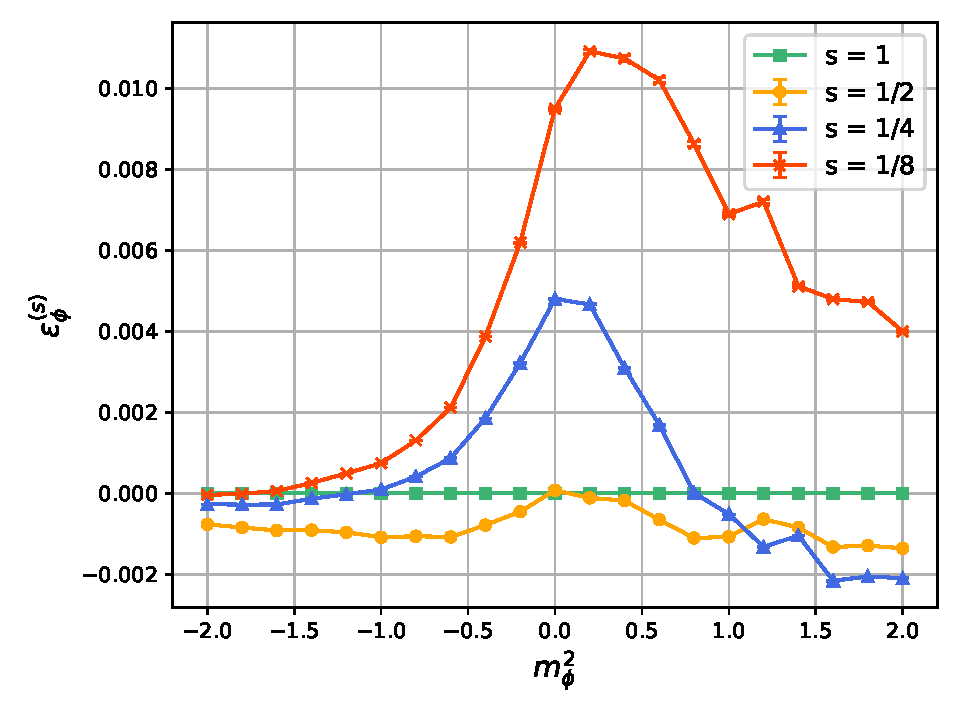
\includegraphics[width=1.0\textwidth]{figures/cooling/mass_scan/deviation.pdf}
        \caption{Absolute magnetisation error}
    \end{subfigure}
    \begin{subfigure}[b]{0.47\textwidth}
        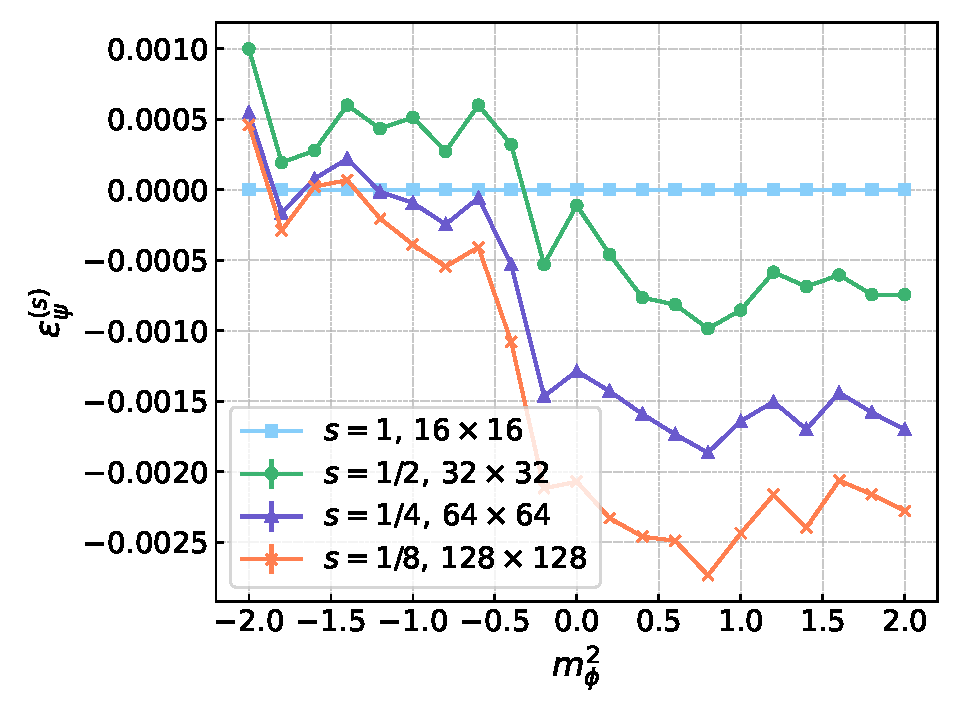
\includegraphics[width=1.0\textwidth]{figures/cooling/mass_scan/deviation_cond.pdf}
        \caption{Chiral condensate error}
    \end{subfigure}
    \caption[Relative error in the cooling procedure at tree level.]{Relative error of the absolute magnetisation and chiral condensate in the cooling procedure for various values of the noise fraction $s$.}
    \label{fig:cooling_deviation}
\end{figure}
\begin{figure}[htp]
    \centering
    \begin{subfigure}[b]{0.47\textwidth}
        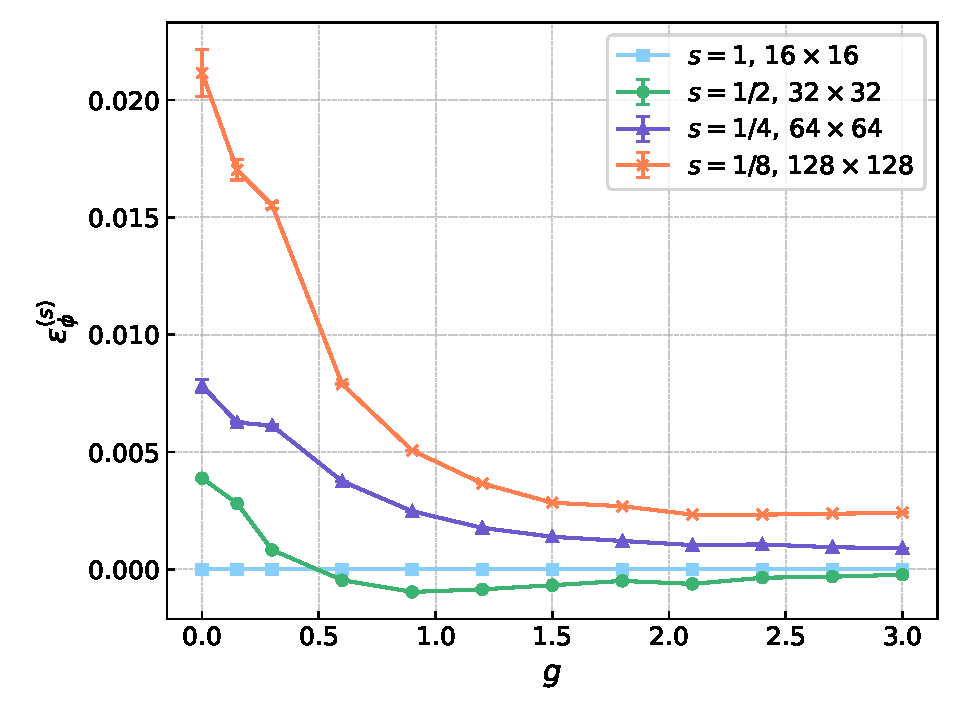
\includegraphics[width=\textwidth]{figures/cooling/yukawa_scan/deviation.pdf}
        \caption{Absolute magnetisation error}
    \end{subfigure}
    \begin{subfigure}[b]{0.47\textwidth}
        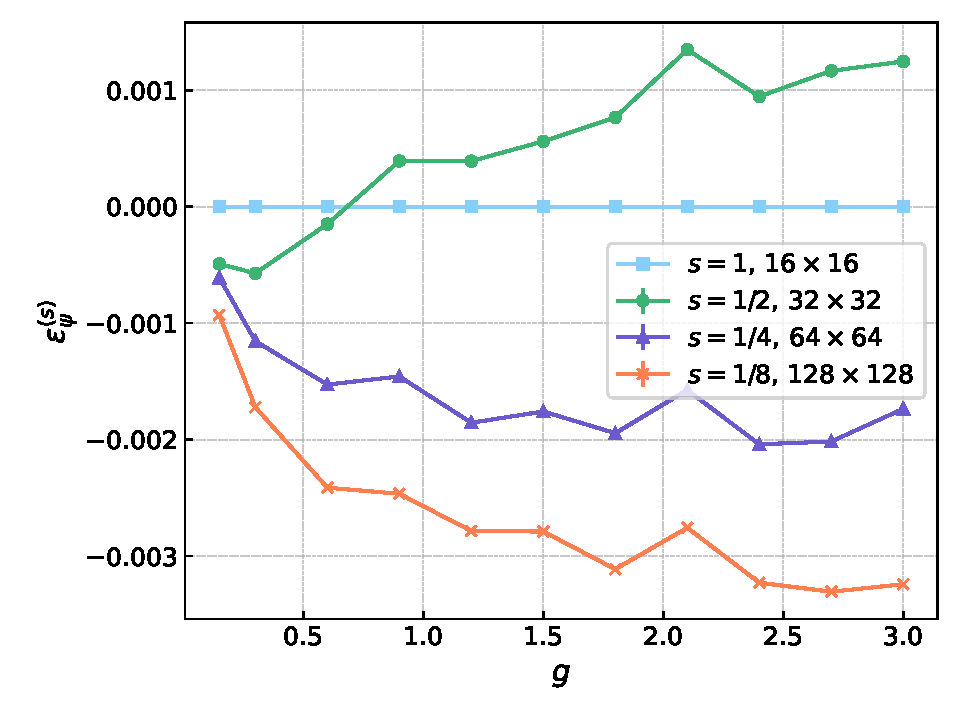
\includegraphics[width=\textwidth]{figures/cooling/yukawa_scan/deviation_cond.pdf}
        \caption{Chiral condensate error}
    \end{subfigure}
    \caption[Relative error in the cooling procedure at tree level.]{Relative error of the absolute magnetisation and chiral condensate in the cooling procedure for various values of the noise fraction $s$.}
    \label{fig:cooling_deviation_yukawa}
\end{figure} \\
Errors obviously increase with successive iterations, since the approximations are multiple. \\
First of all, a tree level rescaling neglects coupling momentum dependencies which do not stem from spacetime rescaling; the assumption is thus justified for high enough cutoffs.  \\
Moreover, the assumption that any change due to a modification of the cutoff can be absorbed by a redefinition of the couplings, is itself non-trivial. In fact, following Wilsonian's RG perspective, as momentum shells are integrated out, 
all the relevant operators, including those not present in the classical action, grow as the cutoff is lowered. As before, the assumption is justified for high enough cutoffs. \\
A quantitative analysis on this aspect was done in \cite{Pawlowski2017CoolingNoise}, where it was proposed a procedure to 
systematically test untill when it is possible to accomodate the cutoff change by a redefinition of the couplings, eventually including also beyond tree level transformations. \\~\\
Finally, we also want to look at more complex observables such as the fermionic physical mass and the bosonic renormalised mass. They are reported in figure \ref{fig:cooling_masses}. 
\begin{figure}[h!]
    \begin{subfigure}{0.47\textwidth}
        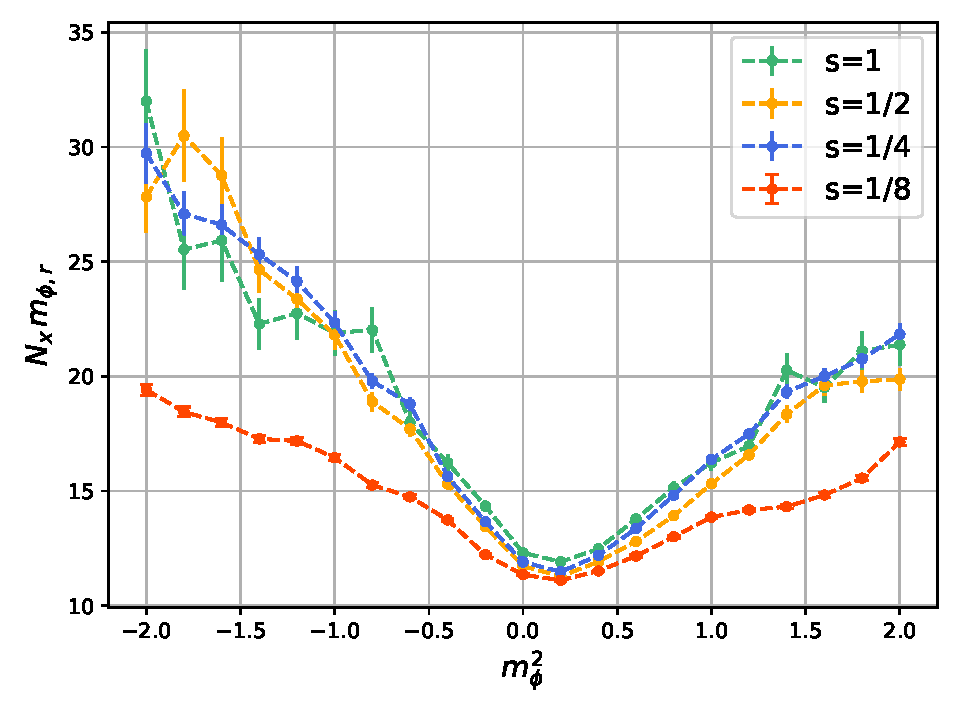
\includegraphics[width=\textwidth]{figures/cooling/mass_scan/mphir.pdf}
        \caption{Renormalised boson mass}
    \end{subfigure}
    \hfill 
    \begin{subfigure}{0.47\textwidth}
        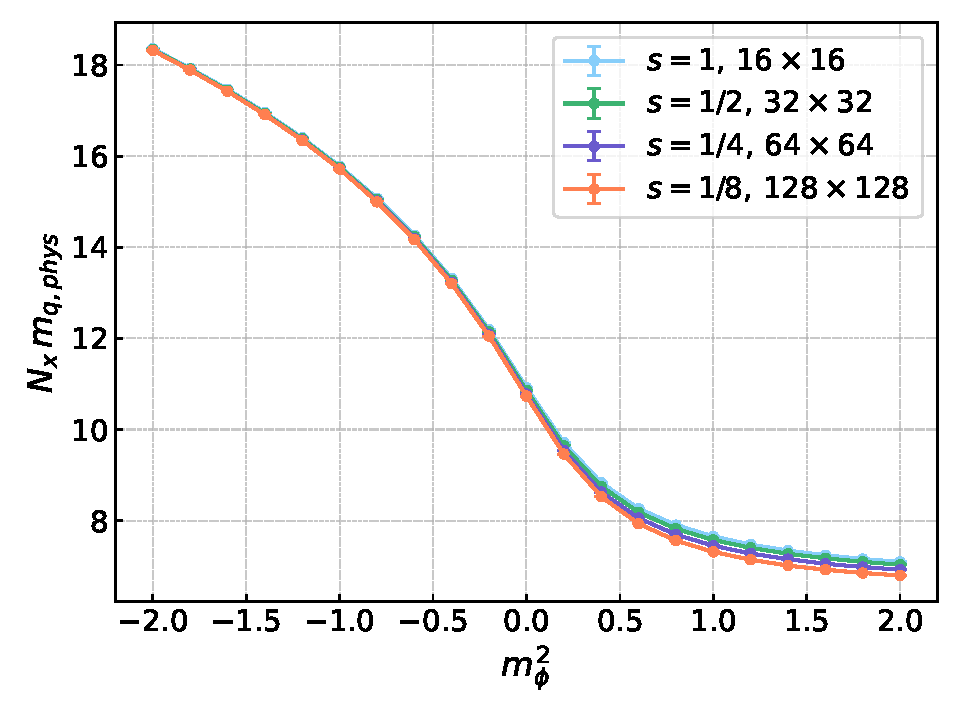
\includegraphics[width=\textwidth]{figures/cooling/mass_scan/mqphys.pdf}
        \caption{Physical quark mass}
    \end{subfigure}
    \caption[Masses in the cooling procedure]{Renormalised bosonic mass $m_{\phi, r}$ and pole fermionic mass $m_{q,\text{phys}}$ for various values of the noise fraction $s$.}
    \label{fig:cooling_masses}
\end{figure}
\begin{figure}[h!]
    \begin{subfigure}{0.47\textwidth}
        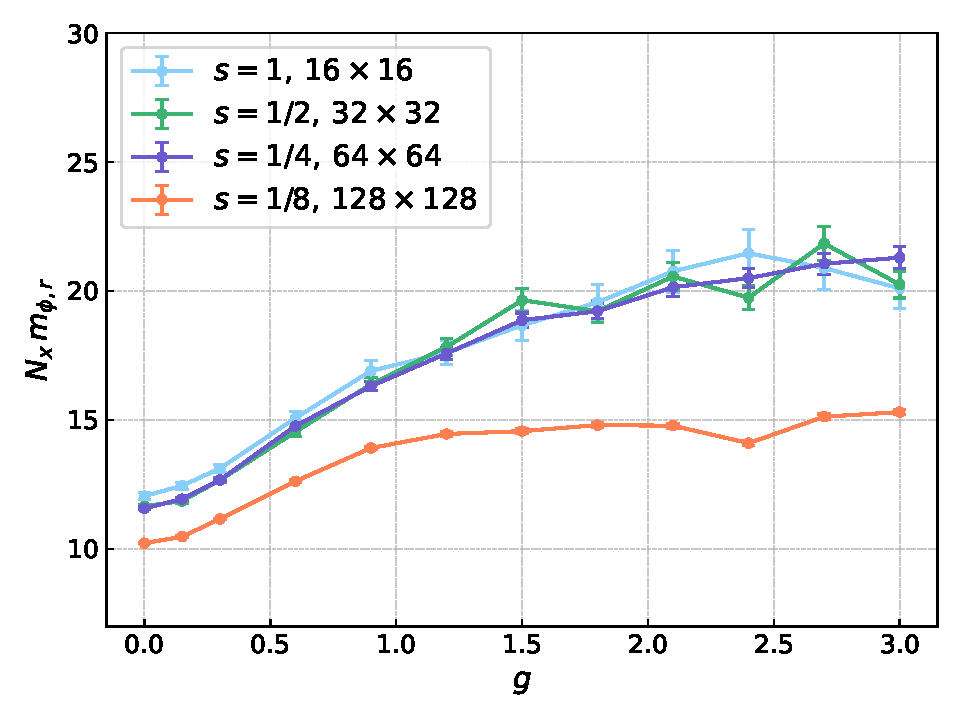
\includegraphics[width=\textwidth]{figures/cooling/yukawa_scan/mphir.pdf}
        \caption{Renormalised boson mass}
    \end{subfigure}
    \hfill 
    \begin{subfigure}{0.47\textwidth}
        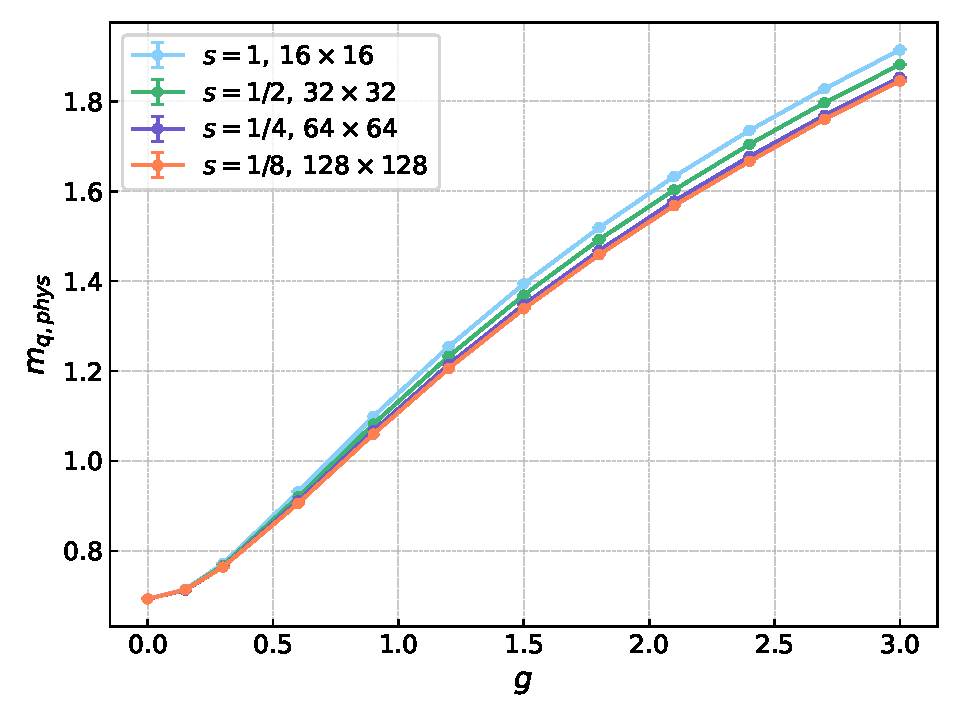
\includegraphics[width=\textwidth]{figures/cooling/yukawa_scan/mqphys.pdf}
        \caption{Physical quark mass}
    \end{subfigure}
    \caption[Masses in the cooling procedure]{Renormalised bosonic mass $m_{\phi, r}$ and pole fermionic mass $m_{q,\text{phys}}$ for various values of the noise fraction $s$.}
    \label{fig:cooling_yukawa_masses}
\end{figure} \\
As one can see, there is a clear deviation for $m_{\phi, r}$ at the third block-spin iteration.
This is indeed a delicate issue that resides in the use of sharp cutoffs to regulate the noise term. In fact, as shown in section \ref{sec:coloured_noise}, the noise-to-noise correlation function expressed in momentum space exhibits an oscillating behaviour described by a Bessel function, which was calculated and shown in figure \ref{fig:bessel}. \\
As a consequence, correlation functions are affected by this behaviour. This holds particularly for the connected two-points function as shown in figure \ref{fig:connected_2ptf}. This explains the big discrepancy encountered in the renormalised mass in figures \ref{fig:cooling_masses} and \ref{fig:cooling_yukawa_masses}. This error cannot be solved
by simply going to higher order correction to the rescaling procedure, but can only be fixed by changing the regulating term, since it is an intrinsic characteristic of the latter. Possible alternative regulators are discusses in \cite{Pawlowski2017CoolingNoise}.
\begin{figure}
    \centering 
    \begin{subfigure}{0.47\textwidth}
        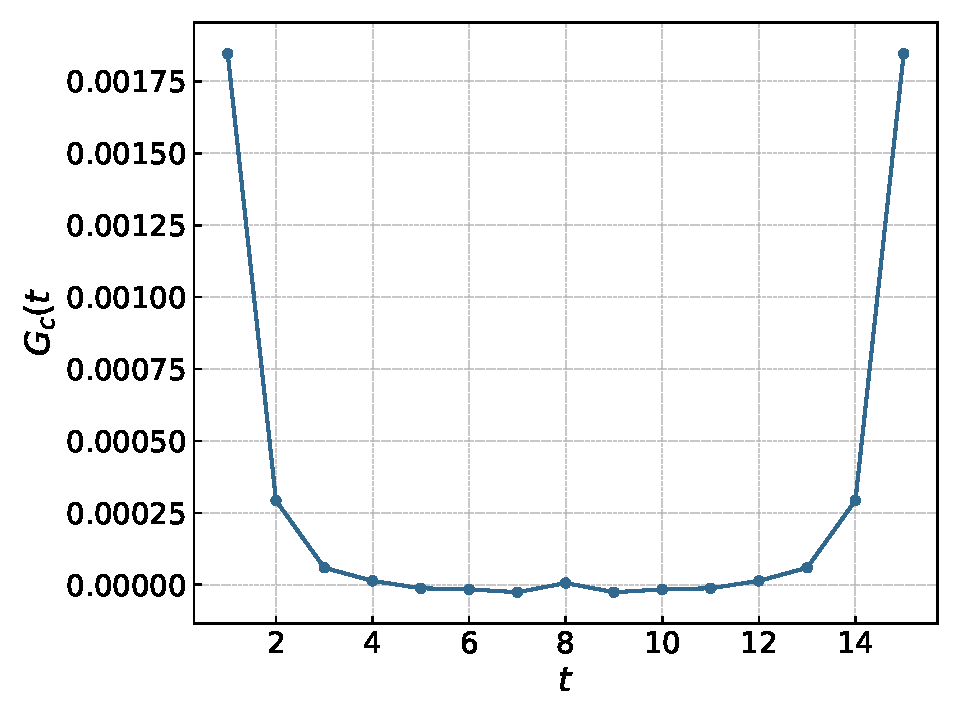
\includegraphics[width=\textwidth]{figures/conn2ptf16.pdf}
    \end{subfigure}
    \begin{subfigure}{0.47\textwidth}
        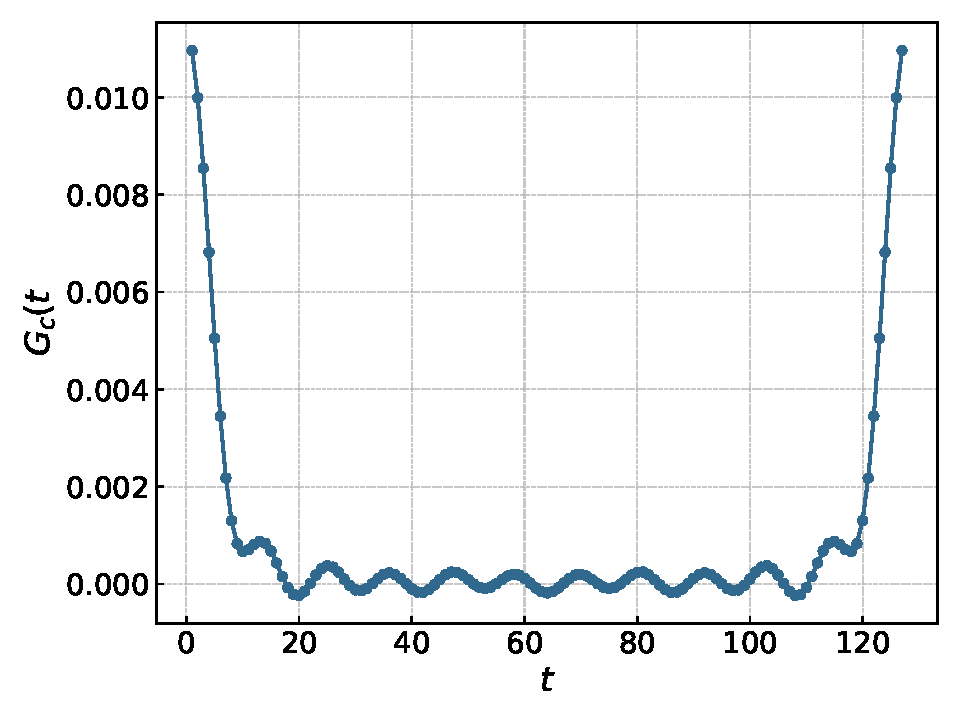
\includegraphics[width=\textwidth]{figures/conn2ptf128.pdf}
    \end{subfigure}
    \caption[Effect of the sharp cutoff on the connected two-points function]{(Left) Connecte two-points function of the original theory on the $16 \times 16$ lattice. (Right) Connected two-points function after three block spin-iterations at cutoff fraction $s=1/8$, on a $128 \times 128$ lattice. The use of the sharp cutoff as a regulating function results in a disturbance of the signal of the bosonic two-points function. The Bessel function profile which was shown in figure \ref{fig:bessel} induces errors in the calculation of the renormalised mass.}
    \label{fig:connected_2ptf}
\end{figure} \\
For what concerns the physical quark mass, which also shows some discrepancy for $m_\phi^2 > 0$, we need to investigate further to understand the cause of the problem. \\
Another source of error is the following: since the regulating term applies strictly speaking, only to the noise term, after performing a block-spin transformation the quantum theory is set back at its original scale, while the classical one lies at a finer spacing. \\
Even with the presence of these problems, it is nevertheless remarkable that observables such as the order parameters are not significantly altered in the coarse-graining procedure.